\documentclass[a4paper, 12pt]{article}
\usepackage{geometry}
\usepackage[T1]{fontenc}
\usepackage{lmodern}
\usepackage{microtype}
\usepackage{amsmath, amssymb}
\usepackage[utf8]{inputenc}
\usepackage[USenglish]{babel}
\usepackage[natbibapa]{apacite}
\usepackage{tikz}
\usetikzlibrary{arrows, positioning}
\usepackage{tikz-dependency}
\usepackage{graphicx}
\usepackage{tabularx}
\usepackage{booktabs}
\usepackage{xcolor}
\usepackage{hyperref}
\usepackage{linguex}

%\newcommand{\ddt}[2]{\frac{\mathrm{d}{#1}}{\mathrm{d}{#2}}}
\newcommand{\ddt}[1]{\frac{\mathrm{d}{#1}}{\mathrm{d}t}}
\newcommand{\todo}[1]{\textcolor{red}{\textbf{TODO: #1}}}

\title{Mparse: A new framework for self-organized, incremental sentence
    comprehension}
%\author{Garrett Smith}

\begin{document}
\maketitle

\begin{abstract}
In the last thirty years, there have been a number of attempts to explain human
sentence processing as a self-organizing process, where a parse for a whole
sentence emerges purely through local, word-word interactions. Previous
attempts have typically used opaque mathematical formalisms
and/or failed to account for important reading time data, and so other
approaches (based on rule-based parsing systems) have remained the focus of
much research in sentence processing. Here, we present a new framework for
self-organized sentence parsing that improves over previous implementations and
opens the door to highly detailed empirical predictions. We test the new model,
called \emph{mparse}, on three important reading time effects using English
materials: garden paths, local coherence, and the ambiguity advantage.
Mparse successfully reproduces these effects and demonstrates the promise of
its more tractable mathematical framing. We hope that the framework will
stimulate new experimental and modeling work.
\end{abstract}

%\tableofcontents



\section{Introduction}
Self-organization of syntactic structures---the idea that a parse of a whole
sentence can arise solely through interactions between pairs of words---has
been floating around in the sentence processing literature for at least 30
years, starting with \citet{kempen1989incremental}. Under self-organization,
the global parse is not constrained to be completely grammatical as in most
other theories of sentence processing. Instead, globally coherent parses arise
through local optimization: If there are two alternative ways of integrating a
word into the preceding structure, one grammatical and one ungrammatical, the
grammatical one is more likely to form, but the ungrammatical one is not
prevented from forming. Local feedback loops reinforce structures as they form,
so if the system ends up in a grammatical state, it is likely to stick with it.
But the same thing can happen if the system begins building a less than optimal
state, which can lead to processing difficulty.  Overall, self-organization
says that human sentence processing is guided by grammatical rules without
being bound by them.

This assumption contrasts with the typical assumption that people
only entertain grammatical structures when comprehending sentences (e.g.,
surprisal theory and its extensions, \citealt{hale2001probabilistic,
    levy2008expectation, levy2008noisy, futrell2017noisy, futrell2020lossy};
and others \citealt{gibson2006interaction, hale2011what}). While these theories
have been largely successful in explaining and predicting sentence
comprehension behavior, the restriction to fully grammatical parses makes
explaining certain facts difficult. For example, reading sentences with
ungrammatical subject-verb number agreement is made less difficult if the sentence
contains a non-subject distractor noun that does agree with the verb in number
\citep{dillon2013contrasting, lago2015agreement, wagers2009agreement,
    pearlmutter1999agreement}. Explaining this fact either requires erroneous retrieval of the
distractor noun from memory \citep{jaeger2017similarity, lewis2005activation,
vasishth2019computational} or the construction of an ungrammatical parse
\citep{smith2018self, smith2021encoding}. A second finding that is difficult to
explain using strictly grammatical parsing is local coherence effects, which
seem to require that people entertain ungrammatical structures during sentence
comprehension \citep{tabor2004effects,
    paape2015local, konieczny2005psychological, konieczny2009local}.
Self-organization-based models naturally allow for ungrammatical states because
of the purely local nature of word-word interactions.
Self-organization-based models have also had success in fitting other sentence
processing effects, including length or ``digging-in'' effects in garden paths
\citep{tabor2004evidence}, number agreement with pseudopartitive subjects
\citep{smith2018self}, encoding interference effects in subject-verb number
agreement \citep{smith2021encoding}, and certain effects of aphasia on sentence processing 
\citep{kempen1989incremental, vosse2000syntactic, vosse2009unification}.%in
%addition to local coherence effects \citep{smith2018toward}.%,
%cho2016bifurcation, cho2017incremental, cho2018dynamic}.

Despite these successes, previous implementations of self-organization for
sentence processing have had a number of shortcomings that have prevented
broad-coverage testing of the theory. First, there many (usually hand-tuned)
free parameters \citep{tabor2004evidence, kempen1989incremental,
    smith2018toward, smith2018self}. This is an issue because we do not know
the full range of effects that the models predict and whether they constrain
possible outcomes at all. Models that can predict any effect are not
informative about the mechanisms they purport to explain
\citep{roberts2000how}. Second, papers describing these models often either do
not report reading time predictions \citep{smith2018self}, or the models make
incorrect predictions \citep{kempen1989incremental}. Word-by-word reading times
from self-paced reading and eye-tracking are two of the main sources of data on
how humans comprehend sentences, so a theory of human sentence processing
should be able to explain how particular reading patterns come about. Finally,
previous models are often unable to handle more than one or two sentence types
with a single set of parameters \citep{smith2018self, smith2018toward,
    tabor2004evidence}. This leaves self-organization-based theories open to
the criticism that they will not ``scale up'' to cover other well-known
processing effects \citep[e.g.,][]{bicknell2009model}, let alone be able to
make reading time predictions for arbitrary sentences. These shortcomings, in
combination, call into question the viability of self-organization as a theory
of human sentence comprehension. The self-organizing model presented here,
called mparse\footnote{\citet{vankampen2007stochastic} suggested ``M-equation''
    as a less grandious-sounding  alternative name for the so-called master
    equation that governs the dynamics in the present model (see Appendix A for
    details). The name ``mparse'' is derived from this suggestion, even though
    the term ``M-equation'' has not caught on outside of
    \citeauthor{vankampen2007stochastic}'s book.}, is designed to implement
word-by-word self-organization of syntactic structure while addressing these
concerns. The mathematical formalism of mparse will allow us to make very
detailed reading time predictions and has few free parameters that we can
systematically explore to discover the full range of predictions that the model
can make. We hope that the work reported here will pave a way for future,
large-scale, quantitative comparisons with other approaches, like surprisal
\citep{hale2001probabilistic, levy2008expectation} or cue-based retrieval
\citep{lewis2005activation}.

The paper is structured as follows: First, the components of the new model are
presented along with a description of the moment-by-moment processing dynamics.
We then test mparse on three important sentence processing effects (in English)
to illustrate how the model works: two types of garden paths \citep[NP/S and
NP/Z;][]{sturt1999structural}, local coherence effects \citep{tabor2004effects},
and the ambiguity advantage \citep{vangompel2000unrestricted,
    traxler1998adjunct, vangompel2001reanalysis, vangompel2005evidence}. We
conclude with a discussion of the results, the limitations of the model, and
possibilities for future work.

\section{Incremental parsing in mparse}
Implementing self-organization as a theory of human parsing requires making a
number of choices. Here, we lay out the choices we made about the nature of
grammatical rules, how the model applies the rules, and how word by word
reading times are derived in mparse while explaining how mparse works step by
step. We present each piece in turn.

\subsection{Choices I: Grammar and parser states}
Mparse represents grammatical knowledge using a dependency grammar consisting
of typed, binary dependency links between specific head words and specific
dependent words \citep{hays1964dependency, gaifman1965dependency,
    demarneffe2019dependency}.  (It would also be possible to implement mparse
using other grammar formalisms like a constituency-based context-free grammar.)
The grammar used for the simulations below is given in Table~\ref{tab:gramm}.
The dependency links in the grammar are assumed to be a subset of the
dependencies that a competent user of a language knows, including lexical and
structural ambiguities. A sample dependency parse of a sentence is given in
Fig.~\ref{fig:depex}. Each link has a link harmony, a continuous measure of its
well-formedness \citep[higher harmony means more
well-formed;][]{smolensky1986information}, and each (partial) parse, a
combination of links, has a harmony that is a function of the harmony of the
links (see below). For simplicity, all link harmonies are set to one in this
paper; however, they can also be estimated from a corpus
\citep[e.g.,][]{smith2020principled}.

\begin{table}[hbtp]
\centering
\caption{The grammar used in the simulations below. Direction refers to the
    side of the head that the dependent should be on. Words in brackets were
    not simulated. The harmony of each head-dependent link was set
    to 1.0 for all simulations. Note that \emph{visited} can only take a direct
    object when it is not followed by a comma.}\label{tab:gramm}
\begin{tabularx}{\textwidth}{XXXXr}
\toprule
Sentence type & Dependency & Head & Dependent & Direction \\
\midrule
Garden path & obj & \emph{saw} & \emph{doctor} & right \\
& ccomp & \emph{saw} & \emph{had} & right \\
& nsubj & \emph{had} & \emph{doctor} & left \\
& mark & \emph{had} & \emph{that} & left \\
& obj & \emph{visited} & \emph{doctor} & left \\
& nsubj & \emph{had} & \emph{doctor} & right \\
& advcl & \emph{had} & \emph{visited[,]} & right \\
\midrule
\mbox{Local coherence} & obj & \emph{smiled [at]} & \emph{player} & right\\
& relcl & \emph{player} & \emph{tossed} & right\\
& relcl & \emph{player} & \emph{thrown} & right\\
& nsubj & \emph{tossed} & \emph{player} & left\\
\midrule
Ambiguity \mbox{advantage} & nmod & \emph{driver} & \emph{[of] car} &
right \\
& nmod & \emph{car} & \emph{[of] driver} & right\\
& nmod & \emph{[of] driver} & \emph{[with] \mbox{mustache}} & right\\
& nmod & \emph{son} & \emph{[of] driver} & right\\
& nmod & \emph{son} & \emph{[with] \mbox{mustache}} & right\\
\bottomrule
\end{tabularx}
{\raggedright nsubj = nominal subject; obj = direct object; ccomp = clausal
    complement; mark = relative clause marker; advcl = adverbial clausal
    modifier; relcl = relative clause
    modifier; nmod = nominal modifier \par}
\end{table}

\begin{figure}[hbtp]
\centering
\begin{dependency}[theme=simple, font=\normalsize, label style={font=\normalsize}]
\begin{deptext}[column sep=1em]
The \& cat \& sleeps.\\
\end{deptext}
\depedge{2}{1}{det}
\depedge{3}{2}{nsubj}
\end{dependency}
\caption{Dependency parse for the sentence \emph{the cat sleeps}. Dependency
    types are from the Stanford Universal Dependencies
    \citep{demarneffe2014universal}: det = determiner, nsubj = nominal
    subject.}\label{fig:depex}
\end{figure}

Mparse uses these lexicalized binary dependency relations to create parse
states that correspond to different partial or complete parses of the string so
far. For a string of $w$ words, mparse generates all partial and complete
dependency parses with up to $w - 1$ dependency links using its grammar and
creates a state for each one. There is also a state for the parse in which
there are no dependencies between words, a no-structure state. For example,
consider the following grammar with only two rules: det(cat, the) and
nsubj(sleeps, cat). This grammar can generate a parse of the sentence \emph{the
    cat sleeps}. Fig.~\ref{fig:netex} shows the sequence of states that are
generated when reading that sentence word by word. After reading \emph{the
    cat}, mparse generates two states, one with no dependency links and one
with \emph{the} attached as the determiner of \emph{cat}. After reading
\emph{sleeps}, mparse adds two more states, one where the only dependency is
that of \emph{cat} being the subject of \emph{sleeps} and one with the complete
parse, with both \emph{the} attached as \emph{cat}'s determiner and \emph{cat}
as \emph{sleeps}' subject.%After reading only \emph{the}, there is effectively
%only the no-structure state, plus a dummy state that exists solely for
%mathematical bookkeeping (see Appendix A for details). 

\begin{figure}[htbp]
\centering

A) the

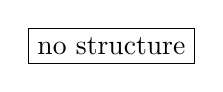
\begin{tikzpicture}[->, >=stealth']
    \tikzstyle{state} = [draw, text centered, align=center]
    \node [state] at (0,0) (nostruct) {no structure};
\end{tikzpicture}

\vspace{0.5cm}
B) the cat

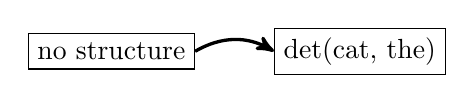
\begin{tikzpicture}[->, >=stealth']
    \tikzstyle{state} = [draw, text centered, align=center]
    \node [state] at (0,0) (nostruct) {no structure};
    \node [state, right =of nostruct] (catthe) {det(cat, the)};
    \draw[bend left, very thick] (nostruct.east) to (catthe.west);
    %\draw[bend left] (catthe.west) to (nostruct.east);
\end{tikzpicture}

\vspace{0.5cm}
C) the cat sleeps

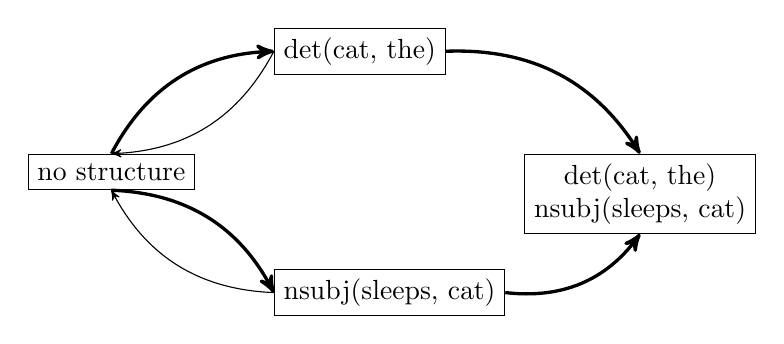
\begin{tikzpicture}[->, >=stealth']
    \tikzstyle{state} = [draw, text centered, align=center]
    \node [state] at (0,0) (nostruct) {no structure};
    \node [state, above right =of nostruct] (catthe) {det(cat, the)};
    \node [state, below right =of nostruct] (nsubj) {nsubj(sleeps, cat)};
    \node [state, below right =of catthe] (full) {det(cat, the)\\nsubj(sleeps,
        cat)};
    \draw[bend left, very thick] (nostruct.north) to (catthe.west);
    \draw[bend left] (catthe.west) to (nostruct.north);
    \draw[bend left, very thick] (catthe.east) to (full.north);
    %\draw[bend left] (full.north) to (catthe.east);
    \draw[bend left, very thick] (nostruct.south) to (nsubj.west);
    \draw[bend left] (nsubj.west) to (nostruct.south);
    \draw[bend right, very thick] (nsubj.east) to (full.south);
    %\draw[bend left] (full.south) to (nsubj.east);
\end{tikzpicture}
\caption{Network representation of the states for \emph{the cat sleeps}. The
    arrows indicate possible transitions, with thicker arrows indicating a
    higher transition rate (higher probability of transitioning per unit time)
    than thinner arrows.}\label{fig:netex}
\end{figure}

Note that as more words are processed, the number of states increases rapidly;
how rapidly depends on what dependencies are allowed by the grammar. Also note
that the states generated by mparse need not be complete parses, and subsets of
the links in the most complete parse (i.e., partial parses) are themselves
separate states of the system.% \citep{kuebler2009dependency,
%    gaifman1965dependency}.  
A number of checks are in place to make
sure that each state is a valid dependency structure. First, core arguments of
head words, e.g., subjects of verbs, determiners of nouns, etc., can only be
used once per head word: A verb can only have one subject, and a noun can only
have one determiner.  Second, each dependent word has at most one head word
governing it. Third, there can be no cycles in the dependency structure, i.e.,
a word cannot be its own dependent or a dependent of one of its dependents.

Finally, for a head-dependent link to be a part of a parse, it must
appear in the grammar. This differs from the assumptions of some other
self-organizing models like \citet{smith2018toward, smith2018self,
    smith2021encoding}, which allow dependency relations between any two words
in a sentence. This divergence from previous self-organizing models has a
number of motivations: very ungrammatical attachments (like attaching the
determiner \emph{the} as the subject of a verb) likely play little to no role
in human sentence processing. Competent language users presumably know that
they can ignore such terrible configurations in most circumstances. Also, it is
simply more practical from an implementation point of view to only use
dependency triples specified in a grammar. One does not need to make decisions about
the harmony values of grammatically impossible configurations, and the
processing dynamics are easier to understand.

The spirit of self-organization is preserved in mparse because the
partial and complete parses are built without considering whether they are
globally coherent. Each individual dependency link must be in mparse's grammar,
but the overall configuration of links need not be mutually consistent. All
possible states that meet the constraints are constructed and considered
without any input from an ``overseer.'' This is the key to explaining local
coherence effects, but it also plays a role in the garden path and ambiguity
advantage examples below.

\subsection{Choices II: State harmonies and transition rates}
Even though mparse considers less than perfect structures, that does not mean
that it treats all states the same. In addition to the link harmonies, whole
states, which consist of zero or more links, are assigned harmony values. The
harmony of a state, as implemented here, is calculated based on three pieces of
information. First, a state has higher harmony if the dependency links in it
have higher harmonies themselves. Since all of the links have a harmony of 1.0,
states that contain more links have a higher harmony than those with fewer
links. Second, in dependency grammar, a complete parse of sequence of $w$ words
has to contain $w - 1$ dependency links. Thus, states with more or less than $w
- 1$ links are penalized by decreasing their harmony. Third, the word order
preferences given by the grammar affect the harmony of a state, as well. If a
word attaches as a dependent of some head word, but the order of the head and
the dependent does not accord with the head's preference, the harmony is
penalized. Finally, dependency length also affects a state's harmony. The more
words between a head and its dependent, the more the state's harmony is
penalized. 

Thus, mparse constructs a discrete state space where each state is a
combination of dependency links between words in the sentence so far. At each
word, new states are added because the new word introduces new ways of
interacting with the words that have already been input. Each state is assigned
a harmony that reflects how well-formed that state is.

We now describe how mparse explores its states and makes reading time
predictions. While processing each word in a sentence, mparse jumps randomly
between states. This jumping around between states constitutes
``parsing'' in mparse. One can think of the model as considering different
analyses of the sentence one by one in a random sequence. It continues this
until it reaches a state whose dependency parse is as complete as possible.
``As complete as possible'' means that a parse contains $w - 1$ dependency
links for a string of $w$ words.\footnote{Sometimes reading the $w$-th word
    leads to a situation where there are no structures possible with $w - 1$
    links. In that case, mparse processes the word until it has built a
    structure with the most dependency links possible given the words so far.}
In general, there can be more than one structure with $w - 1$ links, some more
grammatical, some less grammatical.  But once it has found \emph{some}
state with $w - 1$ links, it reads in the next word.

Mparse jumps stochastically between parse states, but not all jumps are
allowed. It can only move to a new state if the new state differs from the
current state only by a single dependency link. This reflects the assumption of
self-organization where parses emerge through local word-word interactions.
Adding word-word dependencies one at a time embodies this locality. Also, not
all jumps are equally likely: jumps to more well-formed states are more
probable than jumps to less well-formed states (note the different arrow
thicknesses in Fig.~\ref{fig:netex}). More specifically, the transition rate
(probability of jumping per unit time) is higher when jumping from a
low-harmony state to a higher harmony state than in the other direction. A
noise parameter controls how preferable well-formed states are over ill-formed
ones, with low noise resulting in a strong preference for jumping to
well-formed states (compared to ill-formed states) and high noise resulting in
jumps to well- and ill-formed states occurring with more equal probability.

Mathematically, mparse uses a random walk to explore possible parses of a
string of words. The random walk can be described using the master equation
\citep{vankampen2007stochastic}, which describes how the probabilities of a
system being in different discrete states changes in continuous time. This
mathematical formalism was developed in physics and chemistry \citep[see the
papers reprinted in][for examples]{oppenheim1977stochastic}, and its properties
have been well-understood for decades. The master equation is also employed in
an influential model of eye movement control, SWIFT \citep{engbert2005swift,
    engbert2002dynamical}. Here, we take advantage of this
well-established mathematical apparatus for sentence parsing. Appendix A
provides a more detailed description of how the master equation works.
 
\subsection{Choices III: Starting and stopping}
With a set of states and a means of moving between them, we now must specify
how mparse starts and stops processing a word, which will allow us to make
processing time predictions for each word in a sentence. At the first word in a
sentence, there is no dependency structure that mparse can build. Thus, it
just ``builds'' the no-structure state and then inputs the next word. After
that, it adds new states based on how the new word can interact with the
previous one, calculates the harmonies of the new states and the transition
rates between them, and begins jumping around. It stops
processing a word once it reaches an \emph{absorbing state}, a state with $w -
1$ dependency links for a string of $w$ words. The state on the far right of
Fig.~\ref{fig:netex} (C) is an example; it has two dependency links for a
string of three words. The amount of time it takes to
reach any absorbing state is taken to be mparse's prediction for the reading
time of that word.  After reaching an absorbing state, the next word is input,
and the process repeats again until there are no more words to input.

The mathematical formalism of mparse makes it simple to calculate mean
processing time at each word in a sentence using the matrix of transition rates
between states (see Appendix A). The experiments below take advantage of this
and compare the patterns of mean reading time predictions in mparse to the
qualitative patterns of results (ordering of conditions) from existing sentence
comprehension experiments.

\section{Experiments}
In this section, we test mparse on three important classes of processing time
effects in sentence comprehension: the contrast between two types of garden
paths, local coherence effects, and the ambiguity advantage. In order to
understand the full set of predictions mparse can make and to determine whether
there are processing effects which it \emph{cannot} model, we vary its noise
parameter $T$ over a wide range. Simulations of this sort are important in
evaluating how informative the parser is as a theory of sentence processing
\citep{roberts2000how}: If there are parameter settings that allow the model to
predict any possible ordering of condition means, then it cannot be said to
``predict'' the pattern we actually observe in human data. Only if the model
rules out some possible outcomes can it same something about how the process it
models might actually work.\footnote{Mparse contains a second
    free parameter $\tau$ that sets the numerical scale on which processing
    times take place. This parameter does not affect the ordering of conditions
    or standardized effect size measures, so it is set to $1.0$ for all
    simulations. Future work will estimate $\tau$ from reading time corpora to
    put mparse's predictions on the millisecond scale.}

\subsection{Garden paths}
Garden path effects occur when a temporary ambiguity leads to processing difficulty
at disambiguation. They are an empirically well-established sentence comprehension
effect \citep{bever1970cognitive, frazier1978sausage, kimball1973seven}. Here, we focus on the
reported difference in magnitude between two types of garden paths, NP/S and
NP/Z \citep{sturt1999structural, grodner2003against, prasad2019how,
    sturt1997thematic}. In NP/S garden paths, a phrase is temporarily ambiguous
between a noun phrase complement (NP) of an optionally transitive verb and the
subject of a sentential complement of the verb (S): \ex. NP/S ambiguity:
\a.\label{ex:nps-amb} The woman saw the doctor had been drinking.
\b.\label{ex:nps-unamb} The woman saw that the doctor had been drinking.

When a person reads \ref{ex:nps-amb} word by word, the noun phrase \emph{the
    doctor} is temporarily interpreted as the direct object of \emph{saw}. But
once the reader gets to the verb phrase \emph{had been drinking}, it becomes
clear that \emph{the doctor} needs to be the subject of the second verb phrase (see
Fig.~\ref{fig:gpresolve} (A) and (B)).
This reanalysis has been observed to cause reading time slowdowns in the second
verb phrase compared to \ref{ex:nps-unamb} \citep{sturt1999structural,
    grodner2003against, prasad2019how}.
In \ref{ex:nps-unamb}, reading \emph{that} prevents attaching
\emph{the doctor} as \emph{saw}'s direct object, and the correct parse can be
built quickly.

A similar effect occurs in \Next. \ex.\label{ex:npz} NP/Z ambiguity: \a.
\label{ex:npz-amb} Before the woman visited the doctor had been drinking.
\b.\label{ex:npz-unamb} Before the woman visited, the doctor had been drinking.

When a person reads \ref{ex:npz-amb}, it is possible to attach \emph{the
    doctor} as the direct object of \emph{visited}. But after reading \emph{had
    been drinking}, it is clear that \emph{the doctor} has to be the subject of
the second clause instead, leaving \emph{visited} with no (``zero'') complement
(see Fig.~\ref{fig:gpresolve} (C) and (D)). This causes reading time slowdowns
compared to \ref{ex:npz-unamb}, where the comma after \emph{visited} makes it
clear that \emph{the doctor} cannot act as the direct object.

A common assumption is that large changes to existing structure are more costly
than small changes. This assumption is expressed in various reanalysis-based
parsing strategies \citep[see][for discussion]{sturt1999structural} and
parallel models \citep[e.g.,][]{levy2008expectation}. In the case of NP/S and
NP/Z garden paths, this predicts that NP/S ambiguities should be more difficult
to resolve than NP/Z ambiguities. \citet{sturt1999structural} present one way
of making this assumption concrete by arguing that reanalyses that break
established dominance relations are more costly than reanalyses that preserve
them. Consider Fig.~\ref{fig:gpresolve}: (A) and (C) show garden path
structures for the NP/S and NP/Z sentences, respectively; (B) and (D) show the
correct parses after reading the next word \emph{had}. In both (A) and (B), the
main clause verb \emph{saw} dominates the word \emph{doctor} through a chain of
dependencies, both in the garden path state and in the correct parse. However,
the dominance relation between \emph{visited} and \emph{doctor} in (C) has to
be broken in order to build the correct parse in (D).
\citet{sturt1999structural} argue that it is this dominance-breaking reanalysis
that causes the additional slowdown for NP/Z garden paths.

\begin{figure}[htbp]
\begin{dependency}[theme=simple, font=\normalsize, label style={font=\normalsize}]
\begin{deptext}[column sep=1em]
    A) \&  The \& woman \& saw \& the \& doctor \& \dots \\
\end{deptext}
\depedge{3}{2}{det}
\depedge{4}{3}{nsubj}
\depedge{4}{6}{obj}
\depedge{6}{5}{det}
\end{dependency}
\\
\begin{dependency}[theme=simple, font=\normalsize, label style={font=\normalsize}]
\begin{deptext}[column sep=1em]
    B) \&  The \& woman \& saw \& the \& doctor \& had \& \dots \\
\end{deptext}
\depedge{3}{2}{det}
\depedge{4}{3}{nsubj}
\depedge{4}{7}{ccomp}
\depedge{6}{5}{det}
\depedge{7}{6}{nsubj}
\end{dependency}

\begin{dependency}[theme=simple, font=\normalsize, label style={font=\normalsize}]
\begin{deptext}[column sep=1em]
    C) \& Before \&  the \& woman \& visited \& the \& doctor \& \dots \\
\end{deptext}
\depedge{5}{2}{mark}
\depedge{4}{3}{det}
\depedge{5}{4}{nsubj}
\depedge{5}{7}{obj}
\depedge{7}{6}{det}
\end{dependency}
\\
\begin{dependency}[theme=simple, font=\normalsize, label style={font=\normalsize}]
\begin{deptext}[column sep=1em]
    D) \& Before \&  the \& woman \& visited \& the \& doctor \& had \& \dots \\
\end{deptext}
\depedge{5}{2}{mark}
\depedge{4}{3}{det}
\depedge{5}{4}{nsubj}
\depedge{8}{5}{ccomp}
\depedge{7}{6}{det}
\depedge{8}{7}{nsubj}
\end{dependency}
\caption{Dependency parses for NP/S (A and B) and NP/Z ambiguities (C and
    D). A and C show only temporarily viable parses where the noun
    \emph{doctor} attaches as the direct object (obj) of the preceding verb.
    After reading the auxiliary \emph{had}, the garden path parses must be
    revised in order to build the correct parses, shown in B and D. ccomp =
    clausal complement; mark = complementizer or subordinating
    conjunction.}\label{fig:gpresolve}
\end{figure}

We tested mparse on these two types of garden paths. As shown below, mparse
produces the expected difference in effect sizes, but the reasons are somewhat different
than those put forward by \citet{sturt1999structural}.

\subsubsection{Method}
To help in understanding how mparse processes the crucial aspects of the
materials, simplified materials were used (NP/S in \ref{npsshort} and
\ref{npslong}, NP/Z in
\ref{npzshort} and \ref{npzlong}): \ex. \label{ex:gpshortened} \a. \label{npsshort} saw doctor
had (NP/S) \b. \label{npslong} saw that doctor had (NP/S control) \c.
\label{npzshort} visited doctor had (NP/Z) \d. \label{npzlong} visited, doctor
had (NP/Z control)

These simplified materials retain the essential properties of the full
sentences, but they require few enough mparse states that the model's
processing can be easily visualized (see below). Word-by-word model output for
the full sentences in \LLast is provided in Appendix B. Mean reading times from
mparse were calculated using the grammar shown in Table~\ref{tab:gramm}. 

\subsubsection{Results and discussion}






The mean processing times at the final words in \ref{ex:gpshortened} are plotted in
Fig.~\ref{fig:gp-times}. For all values of the noise parameter $T$, the garden
path conditions (labeled ``ambiguous'') are processed more slowly than the
unambiguous control conditions. Mparse thus reproduces one of
the foundational reading time effects in sentence processing research. The
mean processing time curves for both garden path conditions are identical, so
only the NP/Z curve is visible.

\begin{figure}[htbp]
\centering

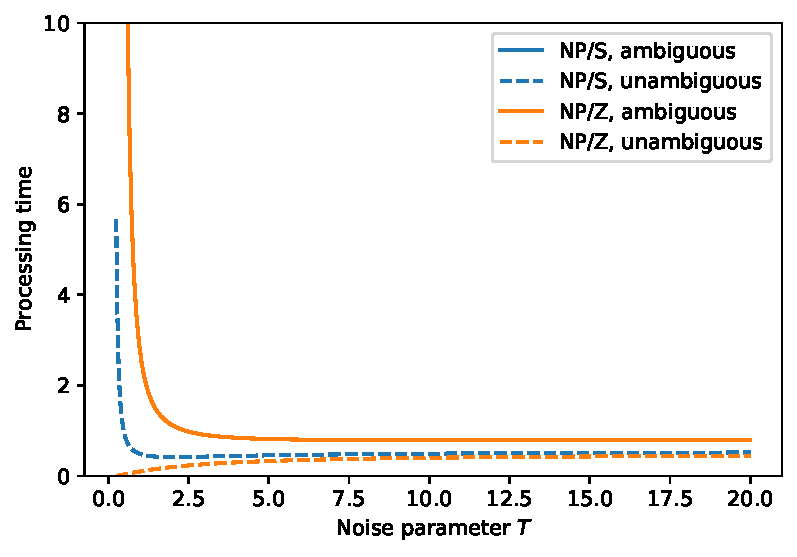
\includegraphics[width= \linewidth]{figures/mparse_intro_gpnoisefig_1.pdf}

\caption{Mean processing times for NP/S and NP/Z garden path materials. The
    processing times for the ambiguous conditions in both types of sentence are
    identical, so only the curve for NP/Z is visible.}\label{fig:gp-times}
\end{figure}

Note that the mean processing time curves for both garden path conditions and
the NP/S control condition diverge to positive infinity as $T$ approaches zero.
This is due to the existence of the dead-end garden path parse states in these
materials (see Fig.~\ref{fig:gpnetworks} (A) through (C)). These states have
relatively low harmony, but their harmony is still higher than the no-structure
state. Recall that the transition rates between states are a function of their
relative harmonies and the noise level. Mparse is less likely to jump from a
higher-harmony state to a lower-harmony state than the other way around, and
this property is exaggerated as the noise level decreases. It becomes less and
less likely that the model will jump out of a garden path state to the
lower-harmony no-structure state. Thus, as the noise decreases, mparse must
spend longer and longer amounts of time in the garden path state (if it jumps
there), which drives the average processing times up sharply. This does not
happen in the NP/Z control case, which does not contain any dead-end states
(see Fig.~\ref{fig:gpnetworks} (D)) because the grammar indicates that
\emph{visited} followed by a comma does not take a direct object.

Obviously, people's reading times in the disambiguating region of a garden path
sentence are not infinite, so we suspect that very low noise levels are not
plausible, although they are included here for completeness. Very low noise
implies a near inability to backtrack or reanalyze a string. We know that
reanalysis is possible in most cases, so in future work, when $T$ is fit to
human data, we expect that the fitted values will not be in this very low
range.

Returning to the difference between the two types of garden paths, the effect
size of the NP/S effect is smaller than the NP/Z effect size for the full range
of $T$ tested. This is also related to the existence of dead-end garden path
states shown in Fig.~\ref{fig:gpnetworks}. For the NP/S conditions (shown in
blue in Fig.~\ref{fig:gp-times}), both the ambiguous and unambiguous conditions
contain dead-end garden path states that slow average reading times.
The NP/S control condition contains a number of different paths (via states
that attach \emph{that} as the relative clause marker of \emph{had}) to the absorbing
state shown on the far right of Fig.~\ref{fig:gpnetworks} (B). If, for example,
mparse happened to be in the no-structure state, there are four possible paths
forward, but only one leads to the dead end. Compare this to the state network
for the ambiguous NP/S condition in Fig.~\ref{fig:gpnetworks} (A), which has only
three ways out of the no structure state. If we further assume that each way
out of the no-structure state is equally probable (which, in general, need not
be the case), the probability of getting garden pathed is 0.25 in the control
condition and 0.33 in the ambiguous condition. Mparse can always get garden
pathed in NP/S materials, but the lower probability of it happening in the
control condition makes its average processing time faster.

The situation is somewhat different for the NP/Z conditions (plotted in orange
in Fig.~\ref{fig:gp-times}. The state network for the ambiguous NP/Z sentence
is identical to that of the ambiguous NP/S condition, so the explanation for
slowed processing is the same. But the NP/Z control condition is different
(compare Fig.~\ref{fig:gpnetworks} (B) and (D)). The NP/Z control condition has
no dead-end garden path state, so it never needs to backtrack to get on a path
to the absorbing state. With NP/S controls, though, mparse can still get
garden pathed, which causes slower average reading times than in the NP/Z
controls. 

A difference in processing times in \emph{control} conditions seems unusual. It
certainly contrasts with the dominance-breaking explanation of
\citet{sturt1999structural}.  Further human experiments will be necessary to
determine whether this prediction of the model can be
confirmed.\footnote{\citet{grodner2003against} found a similar \emph{numerical}
    pattern in some of their materials (see their Appendix B): The control
    conditions for the NP/S sentences were slower than the controls for NP/Z.
    However, this did not hold in \citet{sturt1999structural} or
    \citet{keller2009timing}, so new, higher-powered human experiments are
    needed to test mparse's prediction.}

\begin{figure}[htbp] \centering

A) [woman] saw doctor had\dots

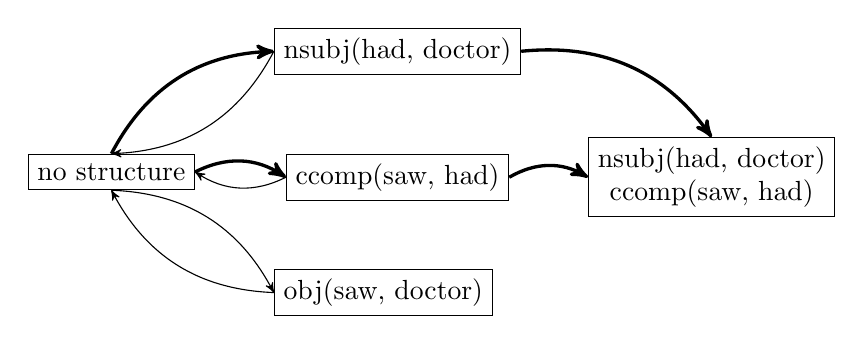
\begin{tikzpicture}[->, >=stealth'] \tikzstyle{state} = [draw, text centered,
    align=center] \node [state] at (0,0) (nostruct) {no structure}; \node
    [state, above right=of nostruct] (haddoc) {nsubj(had, doctor)};
    \node [state, below=of haddoc] (sawhad) {ccomp(saw, had)};
    \node [state, right=of sawhad] (corr) {nsubj(had, doctor)\\ccomp(saw, had)};
    \node [state, below right=of nostruct] (npsgp) {obj(saw, doctor)};
    \draw[bend left, very thick] (nostruct.north) to (haddoc.west);
    \draw[bend left] (haddoc.west) to (nostruct.north);
    \draw[bend left, very thick] (nostruct.east) to (sawhad.west);
    \draw[bend left] (sawhad.west) to (nostruct.east);
    \draw[bend left] (nostruct.south) to (npsgp.west);
    \draw[bend left] (npsgp.west) to (nostruct.south);
    \draw[bend left, very thick] (haddoc.east) to (corr.north);
    %\draw[bend left] (corr.north) to[looseness=0.75] (haddoc.east);
    \draw[bend left, very thick] (sawhad.east) to (corr.west);
    %\draw[bend left] (corr.west) to (sawhad.east);
\end{tikzpicture}

\vspace{0.5cm}
B) [woman] saw that doctor had\dots

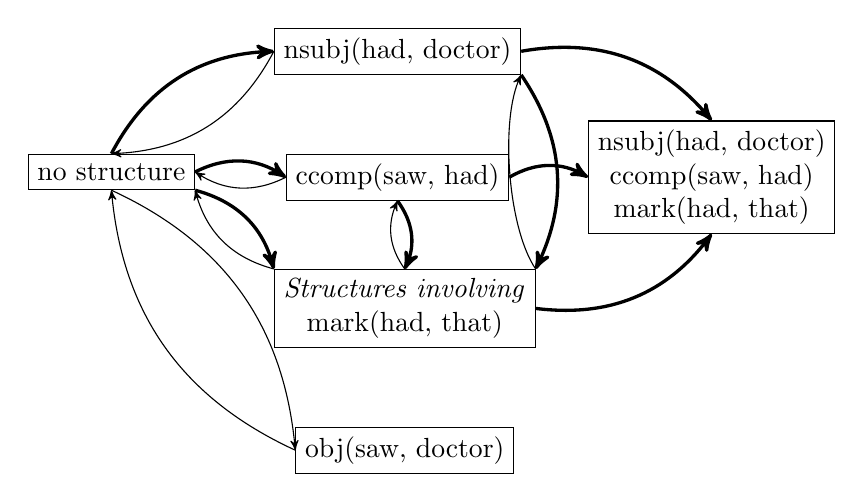
\begin{tikzpicture}[->, >=stealth']
    \tikzstyle{state} = [draw, text centered, align=center]
    \node [state] at (0,0) (nostruct) {no structure};
    \node [state, above right=of nostruct] (haddoc) {nsubj(had, doctor)};
    \node [state, below=of haddoc] (sawhad) {ccomp(saw, had)};
    \node [state, right=of sawhad] (corr) {nsubj(had, doctor)\\ccomp(saw,
        had)\\mark(had, that)};
    \node [state, below right=of nostruct] (thats) {\emph{Structures
            involving}\\mark(had, that)};
    \node [state, below =of thats] (npsgp) {obj(saw, doctor)};
    \draw[bend left, very thick] (nostruct.north) to (haddoc.west);
    \draw[bend left] (haddoc.west) to (nostruct.north);
    \draw[bend left, very thick] (nostruct.east) to (sawhad.west);
    \draw[bend left] (sawhad.west) to (nostruct.east);
    \draw[bend left] (nostruct.south) to (npsgp.west);
    \draw[bend left, very thick] (nostruct.south east) to (thats.north west);
    \draw[bend left] (thats.north west) to (nostruct.south east);
    \draw[bend right, very thick] (thats.east) to (corr.south);
    %\draw[bend left] (corr.south) to (thats.east);
    \draw[bend left, very thick] (haddoc.south east) to (thats.north east);
    \draw[bend left] (thats.north east) to[looseness=0.65] (haddoc.south east);
    \draw[bend left, very thick] (sawhad.south) to (thats.north);
    \draw[bend left] (thats.north) to (sawhad.south);
    \draw[bend left] (npsgp.west) to (nostruct.south);
    \draw[bend left, very thick] (haddoc.east) to (corr.north);
    %\draw[bend left] (corr.north) to[looseness=0.65] (haddoc.east);
    \draw[bend left, very thick] (sawhad.east) to (corr.west);
    %\draw[bend left] (corr.west) to (sawhad.east);
\end{tikzpicture}

\vspace{0.5cm}
C) [before woman] visited doctor had\dots

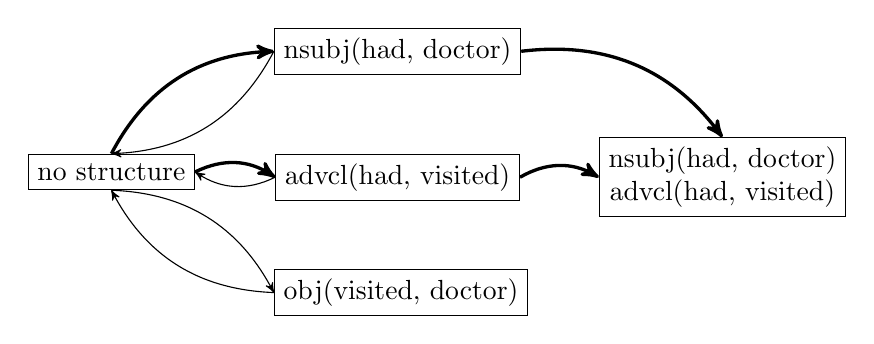
\begin{tikzpicture}[->, >=stealth']
    \tikzstyle{state} = [draw, text centered, align=center]
    \node [state] at (0,0) (nostruct) {no structure};
    \node [state, above right=of nostruct] (visdoc) {nsubj(had, doctor)};
    \node [state, below=of visdoc] (hadvis) {advcl(had, visited)};
    \node [state, right=of hadvis] (corr) {nsubj(had, doctor)\\advcl(had, visited)};
    \node [state, below right=of nostruct] (npzgp) {obj(visited, doctor)};
    \draw[bend left, very thick] (nostruct.north) to (visdoc.west);
    \draw[bend left] (visdoc.west) to (nostruct.north);
    \draw[bend left, very thick] (nostruct.east) to (hadvis.west);
    \draw[bend left] (hadvis.west) to (nostruct.east);
    \draw[bend left] (nostruct.south) to (npzgp.west);
    \draw[bend left] (npzgp.west) to (nostruct.south);
    \draw[bend left, very thick] (visdoc.east) to (corr.north);
    %\draw[bend left] (corr.north) to[looseness=0.75] (visdoc.east);
    \draw[bend left, very thick] (hadvis.east) to (corr.west);
    %\draw[bend left] (corr.west) to (hadvis.east);
\end{tikzpicture}

\vspace{0.5cm}
D) [before woman] visited, doctor had\dots

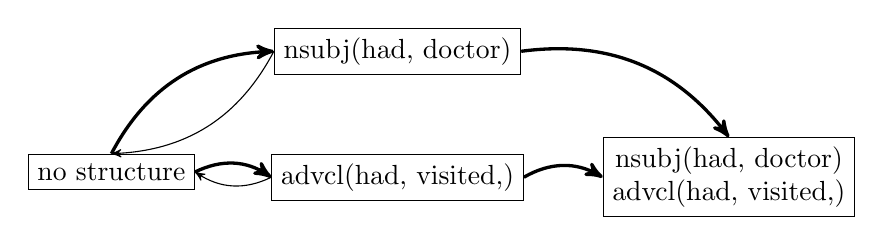
\begin{tikzpicture}[->, >=stealth']
    \tikzstyle{state} = [draw, text centered, align=center]
    \node [state] at (0,0) (nostruct) {no structure};
    \node [state, above right=of nostruct] (visdoc) {nsubj(had, doctor)};
    \node [state, below=of visdoc] (hadvis) {advcl(had, visited,)};
    \node [state, right=of hadvis] (corr) {nsubj(had, doctor)\\advcl(had, visited,)};
    \draw[bend left, very thick] (nostruct.north) to (visdoc.west);
    \draw[bend left] (visdoc.west) to (nostruct.north);
    \draw[bend left, very thick] (nostruct.east) to (hadvis.west);
    \draw[bend left] (hadvis.west) to (nostruct.east);
    \draw[bend left, very thick] (visdoc.east) to (corr.north);
    %\draw[bend left] (corr.north) to[looseness=0.75] (visdoc.east);
    \draw[bend left, very thick] (hadvis.east) to (corr.west);
    %\draw[bend left] (corr.west) to (hadvis.east);
\end{tikzpicture}
\caption{Network representation of the states for the reduced forms in
    \protect\Last. The arrows indicate possible transitions, with the thicker
    arrows indicating a higher transition rate than the thinner arrows. The
    state labeled ``Structures involving mark(had, that)'' in B) conflates
    multiple parse states where \emph{that} attaches as the relative clause marker of
    \emph{had}. Note the lack of a dead-end state in D).}\label{fig:gpnetworks}
\end{figure}

\subsection{Local coherence effects}
Local coherence effects are one of the main motivations for considering
self-organization as a theory of sentence comprehension
\citep{tabor2004effects}. \citeauthor{tabor2004effects} considered sentences
like \Next: \ex. \a. The coach smiled at the player who was thrown the frisbee.
\b. The coach smiled at the player thrown the frisbee. \c. The coach
smiled at the player who was tossed the frisbee. \d. The coach smiled at the
player tossed the frisbee.

Note that \Last (a-b) and \Last (c-d) have all have similar meanings: there is
a frisbee player who caught a frisbee, and the coach smiled at that player. The
(b) and (d) examples contain the reduced relative clause \emph{\dots
    tossed/thrown the frisbee}, which should elicit longer reading times due to
the low frequency of that structure compared to the non-reduced forms in (a)
and (c). \Last (d) contains the string \emph{\dots the player tossed
    the frisbee}. If this string appeared on its own, it would be a perfectly
grammatical main clause with \emph{the player} attaching as the subject of the
verb \emph{tossed}. But in the context of the preceding sentence, this analysis
is not possible; the phrasal verb \emph{smile at} cannot take a complete
sentence as its complement.

\begin{figure}[htbp]
\begin{dependency}[theme=simple, font=\normalsize, label style={font=\normalsize}]
\begin{deptext}[column sep=1em]
    A) \& smiled at \& the \& player \& thrown \& \dots\\
\end{deptext}
\depedge{2}{4}{obj}
\depedge{4}{3}{det}
\depedge{4}{5}{relcl}
\end{dependency}
\\
\begin{dependency}[theme=simple, font=\normalsize, label style={font=\normalsize}]
\begin{deptext}[column sep=1em]
    B) \& smiled at \& the \& player \& tossed \& \dots\\
\end{deptext}
\depedge{2}{4}{obj}
\depedge{4}{3}{det}
\depedge{4}{5}{relcl}
\depedge[edge below]{5}{4}{nsubj}
\depedge[edge below]{4}{3}{det}
\end{dependency}
\caption{Dependency parses for the local coherence materials in \protect\Last.
    The locally coherent parse in (B) is shown below the words of the sentence.
    relcl = relative clause modifier.}\label{fig:gpresolve}
\end{figure}

Theories in which only globally grammatical analyses are considered would not
predict a difference in processing times between \Last (b) and (d). However,
self-organizing theories do because they allow merely locally acceptable
structures to compete with globally grammatical ones.
\citet{tabor2004effects} found self-paced reading times were elevated for both
\Last (b) and (d) (compared to the control sentences (a) and (c)) and that (d)
was processed even more slowly than (b).  This effect, which  has been
replicated a number of times \citep{levy2009eye, mueller2019effect,
    konieczny2005psychological, konieczny2009local, paape2015local,
    kamide2018influence, christianson2017why}, is taken as evidence for the
ungrammatical analysis of \emph{\dots the player tossed the frisbee} competing
with the globally grammatical parse, causing slowed reading times.

%Local coherence effects cannot be explained if only fully consistent parses of
%the whole sentence are considered. 
Theories that posit only grammatical structures have attempted to explain local
coherence through noisy-channel reinterpretation of the input string
\citep{levy2008noisy, levy2009eye} or through costly integration of bottom-up
parse formation with top-down global monitoring \citep{bicknell2009model,
    gibson2006interaction, morgan2010bottom}.  While these theories merit
further discussion, we focus here on understanding how mparse explains local
coherence. We do note that self-organizing theories have the benefit of
parsimony in explaining local coherence effects, as the ungrammatical
competitor parses arise naturally via self-organization, and additional
mechanisms to not need to be added in order to explain the experimental
results.

\subsubsection{Method}
To help in understanding how mparse processes the
crucial aspects of the materials, abbreviated forms were used: \ex. \a.
smiled-at player who was thrown \b. smiled-at player thrown \c. smiled-at
player who was tossed \d. smiled-at player tossed.

These simplified materials retain the essential properties of the full
sentences, but they require few enough mparse states that the model's
processing can be easily visualized (see below). Word-by-word model output for
the full sentences in \LLast is provided in Appendix B. Mean reading times from
mparse were calculated using the grammar shown in Table~\ref{tab:gramm}. 

\subsubsection{Results and discussion}
The reading times at the last words in \Last are shown in
Fig.~\ref{fig:lcresults}. The pattern of results that mparse produces
is qualitatively the same as what \citet{tabor2004effects} observed in
self-paced reading times: The reduced forms are read slower than the
non-reduced forms, and the locally coherent reduced condition is read more
slowly than the non-locally coherent reduced condition.




\begin{figure}[htbp]

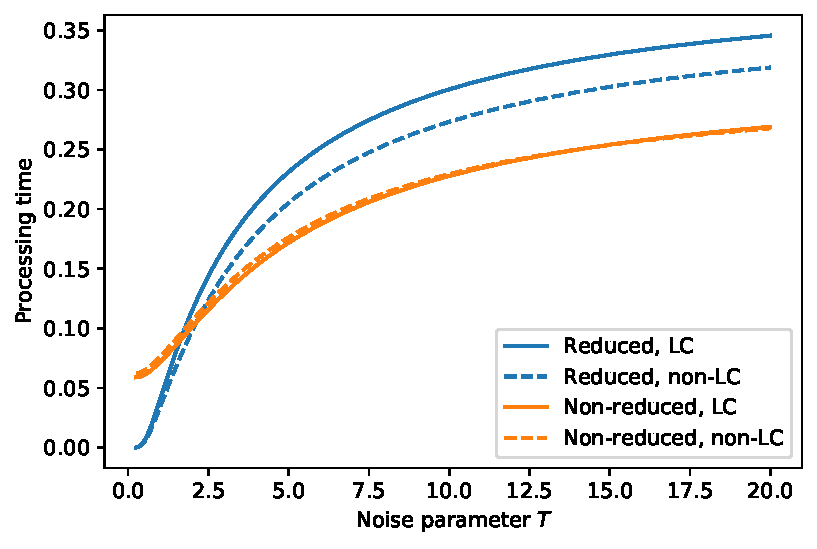
\includegraphics[width= \linewidth]{figures/mparse_intro_lcnoisefig_1.pdf}

\caption{Processing time results from mparse for the local coherence (LC) materials
    in \protect\Last. Mean processing times at \emph{tossed} or \emph{thrown} (y-axis) are
    plotted in arbitrary time units as a function of the noise parameter $T$ on
    the x-axis.}\label{fig:lcresults}
\end{figure}

We can understand how this effect works with the help of
Fig.~\ref{fig:lcnetworks}. Fig.~\ref{fig:lcnetworks} shows the states (in
boxes) that are available after reading \emph{at player tossed/thrown}.
The arrows show the possible transitions between states, with thicker arrows
indicating higher transition rates. The upper network corresponds to the
\emph{thrown} condition. If, for example, we assume that mparse was initialized
in the no-structure state at the far left, it is clear that the model will have
little trouble reaching the absorbing state on the far right which corresponds
to the correct, full dependency parse of the words. The bottom network, which
corresponds to the \emph{tossed} condition contains a dead end. If mparse is
currently in the no-structure state, it is approximately equally likely to jump
to one of the states that lead to the absorbing state or to 
the locally coherent state. If it does jump to the latter, it will have to
backtrack in order to reach the absorbing state with the correct structure.
The possible need for backtracking leads to longer processing times on average
compared to the \emph{thrown} condition.

In the non-reduced conditions (e.g., \emph{\dots who was tossed\dots}), a
similar situation holds. There is a dead-end, locally coherent state in the
\emph{who was tossed} condition but not in the \emph{who was thrown} condition.
However, the dead-end state here has very low harmony because it has too few
links. Thus, mparse is very unlikely to jump to it, and it only has a small
impact on average reading times.

The reason that the non-reduced forms are read more quickly than the reduced
forms for most noise levels is that the state networks for the non-reduced
forms contain more paths to the absorbing state than the networks for the
reduced forms. Having many ways of reaching the absorbing state generally
speeds processing; this was also the explanation for why the NP/S control
condition was faster than the NP/S garden path condition. For very low noise
levels, though, the pattern flips for local coherence: The non-reduced forms are processed more
slowly. This is because some of the additional paths that are available in the
non-reduced forms contain lower-harmony states, specifically, those with
longer-distance dependencies like nsubj(thrown, who). With low noise, the
probability of jumping to lower harmony states drops rapidly, effectively
removing paths to the absorbing state. The dependencies in the reduced
forms are all relatively short, so the effective number of paths to the
absorbing state remains approximately the same, even for low noise.

\begin{figure}[htbp]
\centering

A) smiled-at player thrown\dots

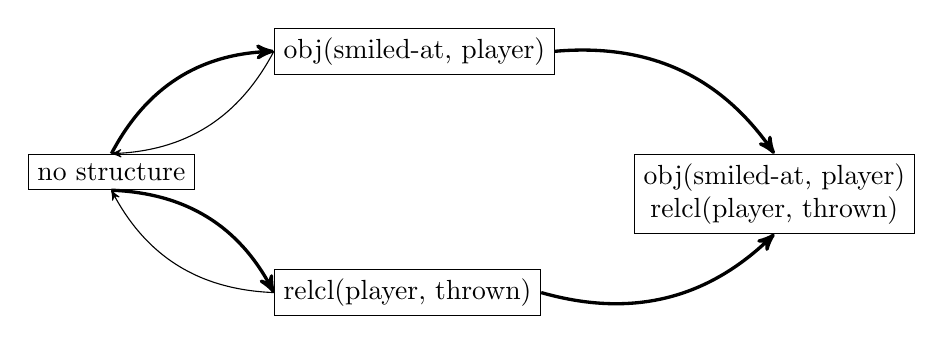
\begin{tikzpicture}[->, >=stealth']
    \tikzstyle{state} = [draw, text centered, align=center]
    \node [state] at (0,0) (5) {no structure};
    \node [state, above right=of 5] (6) {obj(smiled-at, player)};
    \node [state, below right=of 5] (relcl) {relcl(player, thrown)};
    \node [state, below right=of 6] (7) {obj(smiled-at, player)\\relcl(player, thrown)};
    \draw[bend left, very thick] (5.north) to (6.west);
    \draw[bend left, very thick] (6.east) to (7.north);
    \draw[bend left] (6.west) to (5.north);
    %\draw[bend left] (7.north) to (6.east);
    \draw[bend left, very thick] (5.south) to (relcl.west);
    \draw[bend left] (relcl.west) to (5.south);
    \draw[bend right, very thick] (relcl.east) to (7.south);
    %\draw[bend left] (7.south) to (relcl.east);
\end{tikzpicture}

\vspace{0.5cm}
B) smiled-at player tossed\dots

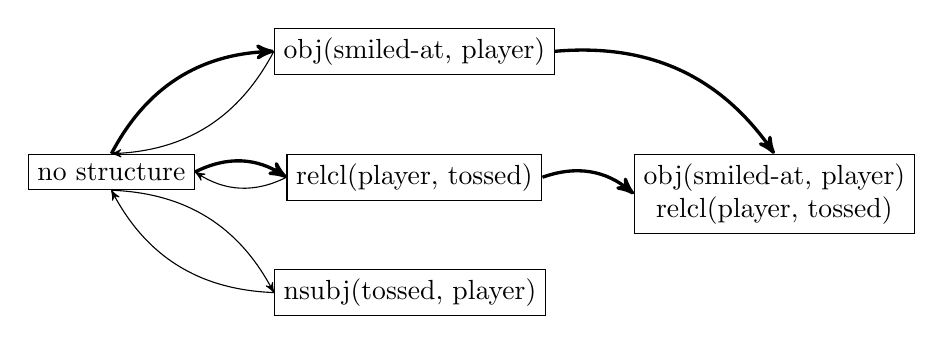
\begin{tikzpicture}[->, >=stealth']
    \tikzstyle{state} = [draw, text centered, align=center]
    \node [state] at (0,-4) (1) {no structure};
    \node [state, above right=of 1] (2) {obj(smiled-at, player)};
    \node [state, below right=of 1] (3) {nsubj(tossed, player)};
    \node [state, below =of 2] (relcl) {relcl(player, tossed)};
    \node [state, below right=of 2] (4) {obj(smiled-at, player)\\relcl(player, tossed)};
    \draw[bend left, very thick] (1.north) to (2.west);
    \draw[bend left] (1.south) to (3.west);
    \draw[bend left, very thick] (2.east) to (4.north);
    \draw[bend left] (2.west) to (1.north);
    \draw[bend left] (3.west) to (1.south);
    %\draw[bend left] (4.north) to (2.east);
    \draw[bend left, very thick] (1.east) to (relcl.west);
    \draw[bend left] (relcl.west) to (1.east);
    \draw[bend left, very thick] (relcl.east) to (4.west);
    %\draw[bend left] (4.west) to (relcl.east);
\end{tikzpicture}
\caption{Network representation of the states for the reduced forms in
    \protect\Last. The arrows indicate possible transitions, with the thicker
    arrows indicating a higher transition rate than the thinner arrows. The
    upper network corresponds to \protect\Last (b), the lower network to
    \protect\Last (d).}\label{fig:lcnetworks}
\end{figure}

An important difference between how mparse processes garden paths and local
coherence becomes apparent when contrasting Figs.~\ref{fig:gp-times} and
\ref{fig:lcresults}. Processing times diverge at low noise settings for garden
paths but not for local coherence materials. The reason is this: For local
coherence, if mparse starts at the no-structure state in the reduced LC
condition, it is approximately equally likely to take any of the three
available transitions to other states.  Two of those transitions lead towards
the absorbing state, and those two have approximately equal harmony and are
therefore approximately equally likely. For NP/S garden paths, e.g.,
the dead-end garden path state and the state with the nsubj(had, doc) link have
approximately equal harmony, so mparse is approximately equally likely to go to
one of them.  But the state with the ccomp(saw, had) link has a longer
dependency, so its harmony is lower than the dead-end or nsubj states. This
means that, for garden paths, the model is more likely to get garden pathed
than it is to take one of the viable paths toward the absorbing state. As the
noise parameter decreases, it becomes both harder to get out of the garden path
state and harder to take a path to the absorbing state. This drives the average
processing times to positive infinity. For slightly higher noise values,
though, garden paths and local coherence effects arise in similar ways; the
model sometimes gets temporarily stuck in a dead-end state that delays it from
reaching the absorbing state and moving on to the next word.

The fact that mparse behaves unlike people in both garden paths (impossibly
long processing times) and local coherence (flipped order of reduced and
non-reduced processing times) suggests that very low noise settings might not
correspond to realistic settings for modeling human behavior. For $T$ values
less than approximately two, the model effectively loses the ability to
reanalyze in garden paths and build a viable parse in local coherence. This
could just be a idiosyncrasy of the model, but it might also suggest that
effective parsing requires some flexibility in parsing. We need to be able to
backtrack through structural choices and press on through temporary difficulty
if we want to comprehend sentences. 

Finally, we highlight the fact that not all possible orderings of condition
means are possible for the local coherence materials. The reduced locally
coherent condition is always processed more slowly than the reduced non-locally
coherent condition. As \cite{roberts2000how} argue, a model that can predict
any possible ordering of conditions is not very informative about the process
it purports to explain. Thus, while mparse does make unrealistic predictions
for some parameter settings, it is still limited in the scope of effects it can
explain.

%\paragraph{Local coherence in German} \todo{Decide whether to keep this or not.
%Probably not.} Local coherence effects have also been
%studied in German \citep{paape2015local, konieczny2005psychological,
%    konieczny2009local}. In German, the local coherence is typically created by
%exploiting the ambiguity of some past participles that are homophonous with
%past-tense singular verbs, e.g.  \Next and \NNext simplified from
%\citet{paape2015local}:
%\exg.Heute wei{\ss} man, dass der General belagerte St\"adte verteidigten.\\
%Today knows one, that the general besieged cities defended.\\
%``Today, we know that the general defended besieged cities.''
%
%\exg. Heute wei{\ss} man, dass die Gener\"ale belagerte St\"adte verteidigte.\\
%Today knows one, that the generals besieged cities defended.\\
%``Today, we know that the generals defended besieged cities.''
%
%In the locally coherent \LLast, the singular \emph{der General} (\emph{the
%    general}) appears to agree in number with the apparently singular verb
%\emph{belagerte} (\emph{beseiged}). This is only locally coherent, though: In
%German, finite verbs must appear clause-finally in embedded clauses, not
%clause-medially, so a competent speaker of German should never posit that
%\emph{belagerte} is a main verb in this context. The globally coherent parse is
%given in the glosses.
%
%Modeling this type of local coherence, where context-dependent word order
%rules are crucial to the effect, requires us to introduce a similar type of
%lexical ambiguity as was needed for garden paths. The word \emph{belagerte}
%would have two sets of dependencies, depending on its part of speech. For its
%reading as a main-clause verb it would have the dependents
%\begin{align*}
%\overleftarrow{\text{\emph{nsubj}}}(\text{\emph{belagerte}, N})\\
%\overrightarrow{\text{\emph{obj}}}(\text{\emph{belagerte}}, N)
%\end{align*}
%whereas as participial adjective it would not introduce any dependents of its
%own (or at least none that are relevant for these sentences). Configurations
%are constructed either with the main-verb interpretation or the adjective
%interpretation; mixes of the two are not allowed.

\subsection{The ambiguity advantage}
Garden paths and local coherence effects are not ambiguous after the whole
sentence has been read. Garden paths are only temporarily ambiguous, and
locally coherent sentences only seem ambiguous when they are not. We have seen
that mparse can explain how these effects can come about in a
self-organization-based model, but it is also important to test the model on truly
ambiguous sentences.

An intuitive prediction for globally ambiguous sentences is that the existence
of multiple viable analyses should slow processing when compared to unambiguous
sentences. However, \citet{traxler1998adjunct} found the
opposite effect in English in the structures in \ref{ambig} \citep[see
also][]{vangompel2001reanalysis, vangompel2005evidence,
    swets2008underspecification}. \ex. \label{ambig} \a. \label{ambig_a} The
driver of the car that had the mustache was pretty cool. \b.  \label{ambig_b}
The car of the driver that had the mustache was pretty cool.  \c.
\label{ambig_c} The son of the driver that had the mustache was pretty cool.
 
They found a speedup in eye-tracking reading times when \emph{that had the
    mustache} could plausibly attach to more than one noun phrase \ref{ambig_c}
compared to unambiguous high attachment in \ref{ambig_a} and the unambiguous
low attachment in \ref{ambig_b}. These findings have been argued to provide
evidence against the idea that ambiguity automatically leads to processing
difficulty. The dependency parses for these materials are shown in
Fig.~\ref{fig:aadeps}.

\begin{figure}[htbp]
\centering
\begin{dependency}[theme=simple, font=\normalsize, label style={font=\normalsize}]
\begin{deptext}[column sep=1em]
    A) \& The \& driver \& of \& the \& car \& with \& the \& mustache\dots\\
\end{deptext}
\depedge{3}{2}{det}
\depedge{3}{6}{nmod}
\depedge{6}{5}{det}
\depedge{6}{4}{case}
\depedge{3}{9}{nmod}
\depedge{9}{8}{det}
\depedge{9}{7}{case}
\end{dependency}

\begin{dependency}[theme=simple, font=\normalsize, label style={font=\normalsize}]
\begin{deptext}[column sep=1em]
    B) \& The \& car \& of \& the \& driver \& with \& the \& mustache\dots\\
\end{deptext}
\depedge{3}{2}{det}
\depedge{3}{6}{nmod}
\depedge{6}{5}{det}
\depedge{6}{4}{case}
\depedge{6}{9}{nmod}
\depedge{9}{8}{det}
\depedge{9}{7}{case}
\end{dependency}

\begin{dependency}[theme=simple, font=\normalsize, label style={font=\normalsize}]
\begin{deptext}[column sep=1em]
    C) \& The \& son \& of \& the \& driver \& with \& the \& mustache\dots\\
\end{deptext}
\depedge{3}{2}{det}
\depedge{3}{6}{nmod}
\depedge{6}{5}{det}
\depedge{6}{4}{case}
\depedge[edge style={dashed}]{6}{9}{nmod}
\depedge[edge style={dashed}]{3}{9}{nmod}
\depedge{9}{8}{det}
\depedge{9}{7}{case}
\end{dependency}
\caption{Dependency structures for materials for the ambiguity advantage. (A)
    shows the high-attachment preference, (B) the low-attachment preference,
    and (C) the globally ambiguous case. The dashed dependency links in (C)
    indicate that either is viable, but only one is possible at a time. Note
    that in the Universal Dependencies, prepositions are dependents (marked
    ``case'') of the nouns they are associated with.}\label{fig:aadeps}
\end{figure}

The unrestricted race model (URM) of \citet{vangompel2000unrestricted} provides an
account for the basic finding. In the URM, the parser starts building all
(fully grammatical) syntactic structures compatible with the input. Whichever
structure is completed first is the one adopted, and the parser moves on. If
the parser builds a structure that turns out to be incompatible with subsequent
input, it must reanalyze the previously built structure, causing a processing
slowdown.  Under the URM, \ref{ambig_c} is faster to process than \ref{ambig_a}
and \ref{ambig_b} because wherever the prepositional phrase beginning with
\emph{with} attaches (to \emph{son} or \emph{driver}), it is compatible with
the rest of the sentence, and so no reanalysis is ever necessary. In
\ref{ambig_a} and \ref{ambig_b}, however, sometimes the \emph{with}-phrase will attach to
an NP incompatible with the rest of the sentence, necessitating reanalysis and
slowing reading times.

The ambiguity advantage is an interesting test case for mparse. Mean processing
times in mparse reflect a complex interplay between the cost of having multiple
reasonably well-formed structural alternatives and the exact structure of state
network that mparse produces for a given sentence. Understanding how mparse
processes globally ambiguous sentences will thus shed further light on the
factors that affect mean processing times in the model.

\subsubsection{Method}
As for the other experiments, simplified materials were used for the ambiguity
advantage in order to make the processing dynamics easier to understand and
visualize (elided words in brackets): \ex. \label{ex:aashort} \a.
\label{aahighshort} driver [of] car [with] mustache \b. \label{aalowshort} car
[of] driver [with] mustache \c. \label{aaambshort} son [of] driver [with]
mustache 

Word-by-word model output for the full sentences in \LLast is provided in
Appendix B. Mean reading times from mparse were calculated using the grammar
shown in Table~\ref{tab:gramm}. 




\subsubsection{Results and discussion}
The mean processing times at the final words in \ref{ex:aashort} are plotted in
the top panel of Fig.~\ref{fig:aa}. Similar to the pattern in total reading
times (eye-tracking) in \citet{traxler1998adjunct}, mean processing times for
the globally ambiguous condition are faster than the high-attachment and
low-attachment conditions.  In addition, mparse predicts that the
high-attachment condition should be read more slowly than the low-attachment
condition. This is because the high-attachment condition involves a
longer-distance dependency between \emph{driver} and its dependent
\emph{mustache}. This lowers the overall harmony structures that contain that
dependency compared to the low-attachment condition, where the same dependency
spans fewer words. This fits with the pattern observed in
\citet{swets2008underspecification} with items with no or superficial
comprehension questions.

\begin{figure}[htbp]

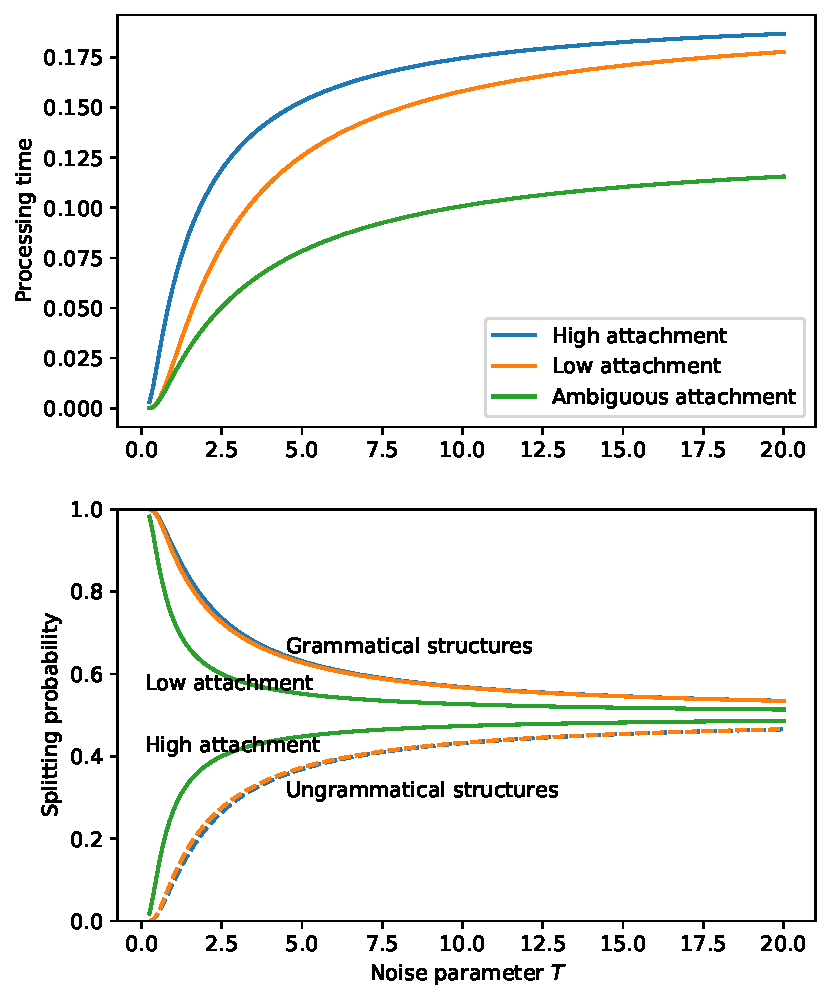
\includegraphics[width= \linewidth]{figures/mparse_intro_aanoisefig_1.pdf}

\caption{Top panel: Mean processing times by condition. Bottom panel: splitting
    probabilities. The dashed curves marked ``ungrammatical'' are parses where
    the first noun attaches as the nominal modifier of the second, in violation
    of the word order preference in the grammar. For the globally ambiguous
    condition in green, both absorbing states are grammatical, although the higher
    harmony of the low-attachment structure leads to a higher splitting
    probability.}\label{fig:aa}
\end{figure}

Fig.~\ref{fig:aanetworks} provides more information about how these results
arise. Fig.~\ref{fig:aanetworks} (A) shows the state network for the
high-attachment preference \ref{aahighshort}. In contrast to the garden path
and local coherence examples, there are now two absorbing states because the
all three sentences are globally ambiguous according to mparse's grammar. One
absorbing state corresponds to the the fully grammatical, correct parse where
\emph{mustache} and \emph{car} are modifiers of \emph{driver}. The other
absorbing state reverses the dependency between \emph{car} and \emph{driver},
with \emph{car} now taking \emph{driver} as its modifier. This violates the
word order preference of the nominal modifier rule of the grammar, so its
overall harmony is lower. The relatively low harmony leads to lower splitting
probability for that state, shown in the lower panel of Fig.~\ref{fig:aa}. The
splitting probabilities are the probabilities that mparse will end up in
different absorbing states.\footnote{When there is only one absorbing state
    (like for garden path and local coherence examples), probability of
    absorption into that state is one.} The state network for the
low-attachment condition \ref{aalowshort}
is similar (with an ungrammatical state where both \emph{car} and
\emph{mustache} attach as nominal modifiers of \emph{driver}); this leads to
similar splitting probabilities.

This illustrates an important property of mparse: Coding the grammar in
binary relations between pairs of words can lead to unexpected and ill-formed
structures being considered. However, unless the noise parameter $T$ is set to
a high value, those states will play only a minor role in parsing, and
grammatical structures will be built with a high probability. The mathematical
formalism behind mparse allows us to explicitly calculate those probabilities
and quantify just how strong an influence extra-grammatical parses can exert.

For the globally ambiguous condition \ref{aaambshort}, both absorbing states
(Fig.~\ref{fig:aanetworks} (B)) have high harmony. The low-attachment structure
(where \emph{mustache} attaches as the dependent of \emph{driver} instead of
\emph{son}) has a slightly higher harmony due to its shorter dependency
lengths, which is also reflected in the slightly higher splitting probability
(Fig.~\ref{fig:aa}, green lines in the lower panel).

\begin{figure}[htbp]
\centering

A) driver [of] car [with] mustache\dots

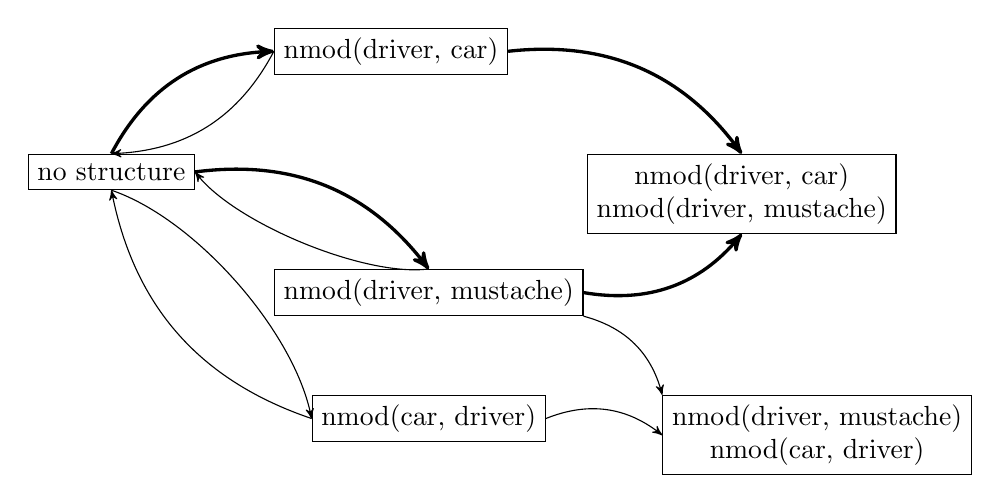
\begin{tikzpicture}[->, >=stealth']
    \tikzstyle{state} = [draw, text centered, align=center]
    \node [state] at (0,0) (5) {no structure};
    \node [state, above right=of 5] (6) {nmod(driver, car)};
    \node [state, below right=of 6] (7) {nmod(driver, car)\\nmod(driver,
        mustache)};
    \node [state, below right=of 5] (8) {nmod(driver, mustache)};
    \node [state, below=of 8] (9) {nmod(car, driver)};
    \node [state, below right=of 8] (10) {nmod(driver, mustache)\\nmod(car, driver)};
    \draw[bend left, very thick] (5.north) to (6.west);
    \draw[bend left, very thick] (6.east) to (7.north);
    \draw[bend left, very thick] (5.east) to (8.north);
    \draw[bend right, very thick] (8.east) to (7.south);
    \draw[bend left] (6.west) to (5.north);
    %\draw[bend left] (7.north) to[looseness=0.75] (6.east);
    \draw[bend left] (8.north) to[looseness=0.65] (5.east);
    \draw[bend left] (8.south east) to (10.north west);
    %\draw[bend right] (7.south) to[looseness=0.65] (8.east);
    %\draw[bend left] (10.west) to (9.east);
    %\draw[bend left] (10.north west) to (8.south east);
    \draw[bend left] (5.south) to[looseness=0.75] (9.west);
    \draw[bend left] (9.west) to (5.south);
    \draw[bend left] (9.east) to (10.west);
\end{tikzpicture}

\vspace{0.5cm}
B) son [of] driver [with] mustache\dots

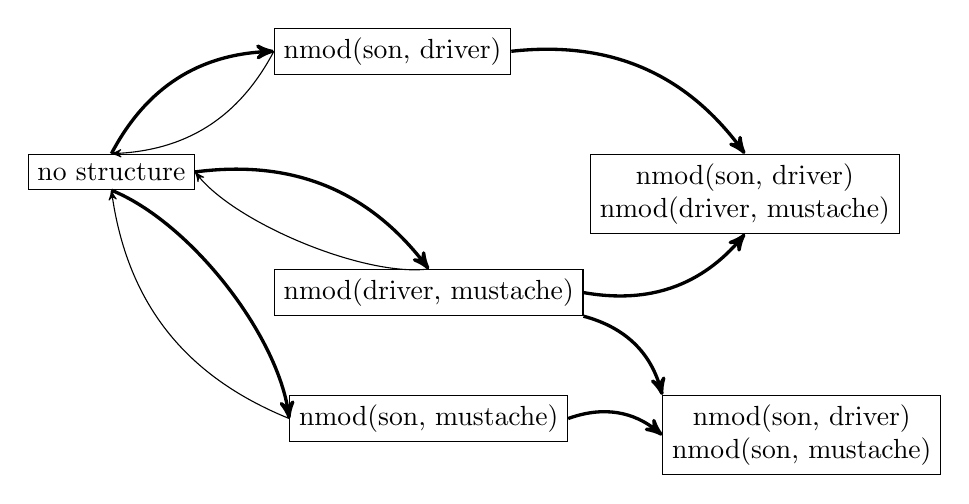
\begin{tikzpicture}[->, >=stealth']
    \tikzstyle{state} = [draw, text centered, align=center]
    \node [state] at (0,0) (5) {no structure};
    \node [state, above right=of 5] (6) {nmod(son, driver)};
    \node [state, below right=of 6] (7) {nmod(son, driver)\\nmod(driver,
        mustache)};
    \node [state, below right=of 5] (8) {nmod(driver, mustache)};
    \node [state, below=of 8] (9) {nmod(son, mustache)};
    \node [state, below right=of 8] (10) {nmod(son, driver)\\nmod(son, mustache)};
    \draw[bend left, very thick] (5.north) to (6.west);
    \draw[bend left, very thick] (6.east) to (7.north);
    \draw[bend left, very thick] (5.east) to (8.north);
    \draw[bend right, very thick] (8.east) to (7.south);
    \draw[bend left] (6.west) to (5.north);
    %\draw[bend left] (7.north) to[looseness=0.75] (6.east);
    \draw[bend left] (8.north) to[looseness=0.65] (5.east);
    \draw[bend left, very thick] (8.south east) to (10.north west);
    %\draw[bend right] (7.south) to[looseness=0.65] (8.east);
    %\draw[bend left] (10.west) to (9.east);
    %\draw[bend left] (10.north west) to (8.south east);
    \draw[bend left, very thick] (5.south) to[looseness=0.75] (9.west);
    \draw[bend left] (9.west) to (5.south);
    \draw[bend left, very thick] (9.east) to (10.west);
\end{tikzpicture}
\caption{Network representation of the states for the simplified forms in
    \protect\Last. The arrows indicate possible transitions, with the thicker
    arrows indicating a higher transition rate than the thinner arrows. The top
    network corresponds to \protect\Last (a) and the lower network to
    \protect\Last (c).}\label{fig:aanetworks}
\end{figure}

These results show that mparse explains the ambiguity effect in a similar
way to the URM. In mparse, multiple paths to high-harmony absorbing states lead
to fast processing times, just as a race process between two well-formed parses
in the URM does. Mparse and the URM are also similar in that both end up with a
single parse at the end of processing a word. Arriving at different parses
takes different amounts of time (in general), and so both models predict
different processing time distributions depending on which parse is built. The
URM has been implemented computationally in \citet{logacev2015multiple} and
\citet{logacev2016understanding}, so future work can compare mparse's
predictions with those of \citeauthor{logacev2015multiple}'s models. We note,
though, that \citeauthor{logacev2015multiple}'s models were meant to capture
task effects first reported by \citet{swets2008underspecification}, where the
ambiguity advantage effect can be attenuated when post-sentence comprehension
questions ask about the ambiguous attachment. Future work must determine how to
incorporate such task effects into mparse. For now, we must be content with
mparse's ability to reproduce the basic effect of \citet{traxler1998adjunct}.

It is also important to note that the low-attachment preference typically seen
in English does not hold in all other languages, and other orderings of the
high, low, and ambiguous attachment conditions have been observed. For example,
\citet{chernova2015syntactic} found a high attachment preference in offline
measures and no ambiguity advantage in self-paced reading and eye tracking in
Russian. \cite{cuetos1988cross} report a similar high-attachment preference in
Spanish. Thus, future cross-linguistic work with mparse might require us to
rethink the inclusion or the weighting of the penalty for longer dependencies, as
the current implementation assumes longer links always result in lower-harmony
structures. This assumption might not hold for languages other than English.

\section{General discussion}
Mparse is a model of incremental sentence parsing in which dependency parses
self-organize. This process is implemented using the master equation formalism
borrowed from physics, chemistry, and biology \citep{oppenheim1977stochastic,
    vankampen2007stochastic, iyer-biswas2016first}. Analysis using the master
equation formalism allows us to determine analytically how probable different
structural analyses are and to make word-by-word reading time predictions. 

We showed that mparse can account for local coherence effects
\citep{tabor2004effects}, the difference in effect size for two types of garden
paths \citep{sturt1999structural}, and the ambiguity advantage
\citep{traxler1998adjunct} for a broad range of parameter settings. Only for
very low noise levels, where the model effectively looses the ability to
reanalyze, do the predicts fail to correspond to established human reading time
effects. Local coherence and garden paths are caused when the model gets
temporarily trapped in isolated ``dead-end'' parses. Mparse thus provides a
unified analysis of two seemingly unrelated sentence comprehension effects.
Mparse reproduces the ambiguity advantage because globally ambiguous structures
offer multiple high-harmony paths to a fully harmonious absorbing state
\citep[similar to the URM;][]{vangompel2000unrestricted}, whereas the high- and
low-attachment conditions contain some paths to low-harmony absorbing states
that take longer to build.

Mparse improves upon previous self-organizing models in a number of ways.
First, it contains only one truly free parameter that controls the noise ($T$;
there is an additional scaling parameter that has no effect on the qualitative
shape of processing time predictions. See Appendix A.). The processing time
effects hold over a wide range of this noise parameter, so hand-picking a value
to demonstrate results was not necessary. Second, mparse correctly predicts
reading time patterns, in contrast to some (but not all) previous
self-organizing models \citep[e.g.,][]{kempen1989incremental, smith2018self}.
Finally, mparse can reproduce local coherence effects, two types of garden
paths, and the ambiguity advantage all using the same set of parameters. In
fact, for the simulations presented here, the model was created once with a
single set of grammar rules and then tested with all constructions while
varying the noise parameter simultaneously for all sentences. This suggests
that mparse could scale up to broad-scale parsing (see future directions below).

A key innovation in mparse is the application of the master equation. This
formalism describes the random-walk parsing process by saying how the
probabilities of different parse states changes in time. The powerful analyses
that this formalism allows \citep{oppenheim1977stochastic,
    iyer-biswas2016first, polizzi2016mean, vankampen2007stochastic} set mparse
apart from many previous self-organization-based models, where the most viable
way of understanding a model was to simulate it many times and see what
happens
\citep{kempen1989incremental, vosse2000syntactic, vosse2009unification,
    tabor2004evidence, smith2018toward, smith2018self, smith2021encoding}.
Indeed, couching mparse's dynamics in this well-understood mathematical
framework allows us to make quantitative reading time predictions, an
improvement over some previous self-organizing models
\citep[e.g.,][]{smith2018self, kempen1989incremental}. Only
the gradient symbolic computation models, perhaps, can be as extensively
analytically investigated as mparse to understand sentence processing effects,
although these models do not allow ungrammatical structures to
form\footnote{Structural blends are possible, that is, superpositions of two or
more grammatical structures. These blends do not resolve to globally incoherent
parses, though \citep{cho2017incremental}.}
\citep{cho2016bifurcation, cho2017incremental, cho2018dynamic,
    tupper2018discrete}.% There is actually much more information about mparse's
%processing dynamics available using the master equation approach; See
%below for additional details. 

%
%\paragraph{Other models} \todo{Need to address the similarities/differences with
%    \citep{hale2011what}.} Possibly include here a mention of how mparse is pretty
%left-corner-y: when a word is read, it brings with it a set of possible
%dependents it might take, its affordances for interacting with upcoming or
%preceding words. Thus, it's not strictly bottom-up avoiding the issues
%therewith \citep{hale2011what, resnik1992left}

Mparse is close in spirit to information theoretic approaches to sentence
processing \citep{hale2016information, hale2003information,
    levy2008expectation}. These approaches have in common that changes in the
probability distribution over structures have a causal effect on processing
times. For entropy reduction \citep{hale2003information}, reading times are
proportional to how much uncertainty has been reduced after reading a new word.
Surprisal theory states that reading times are proportional to the change in
the probability distribution over structures from one word to the next.
Mparse explicitly models the change in the probabilities of different
structures, so it will be possible in future work to calculate entropy and
surprisal values at each word while mparse processes it. Entropy is a summary
statistic of a probability distribution, and time-dependent summary statistics
are simple to calculate using the master equation
\citep[e.g.][]{lu2005kinetics, levy2002eigenvalue}. Surprisal for each word can
be easily calculated as well from as the Kullback-Leibler divergence between the
splitting probabilities at word $w_n$ and word $w_{n+1}$. Thus, it is possible
to make very detailed comparisons between these frameworks and possibly to
derive diverging, testable predictions.

\subsection{Limitations}
Every computational model has limitations. We have tried to be as explicit as
possible about the choices made in implementing mparse, but it is possible that
the successes mparse shows in reproducing existing effects are due to
particular choices. A different grammar formalism, for example could lead to
differently structured state networks, which fundamentally affect processing
time predictions. For example, the fact that the difference in NP/S and NP/Z garden path
effects is driven by differences in the \emph{control} conditions might stem
from our choice of grammar.

The particular form of the harmony function is also a crucial choice. We chose
to penalize parse states if they have long dependencies; this led to diverging
processing time predictions with garden path materials but not with local
coherence materials. Removing that constraint would likely lead to different
garden path results and could cause there to be no difference between NP/S and
NP/Z garden paths in mparse.

We have tried to justify our choices, but others are welcome to question them
and try out different ones. All model data are generated using Python embedded
in the Latex source file for this paper using Pweave \citep{pastell2017pweave},
so our results can be easily reproduced. The source code for mparse and the
Latex source for this paper are available at \url{https://osf.io/k6rnx/}.

In this paper, we have focused on mean processing times as a function of the
noise parameter. But as \citet{roberts2000how} discuss, the variability in the
human data plays just as important a role in evaluating a model as the model's
predictions do. If the human data are too noisy or variable, model fit is not
very informative because we do not actually know much about how people perform.
Future work with mparse should compare the range of model predictions to the
range of effects from experiments, as was done in
\citet{vasishth2018statistical} and \citet{jaeger2019interference} for the
cue-based retrieval model of \citet{lewis2005activation} in order to determine
the extent to which mparse's predictions overlap with the range of reading
times humans produce.

Finally, mparse does not implement any kind of prediction, at least not in the
sense of prediction where structure or even particular lexical items are
activated before they are encountered in the input. Examples of participants
looking at referents of words in anticipation of words not yet encountered
\citep[e.g.,][]{altmann1999incremental, kukona2014lexical} cannot be
explained with the current form of mparse. Additional work is needed to
determine whether prediction in this sense can be added to mparse.
%\textbf{Another limitation:} Meant as a model of self-paced reading
%\citep{just1982paradigms} or possibly early eye-tracking measures (e.g. first
%pass reading times). No mechanism for initiating regressions, z.B.

\subsection{Future directions}
As mentioned above, this paper only scratches the surface of the mathematical
details that can be extracted from mparse's master equation formalism. Among
others, full processing time probability density functions conditional on the
initial and absorbing states can be derived \citep{iyer-biswas2016first,
    polizzi2016mean, valleriani2008dwell, valleriani2014unveiling}. This will
generate new predictions about what reading times at each word in a sentence
should look like given which parse was built at the previous word and which
parse is built at the current word. Also, moment-by-moment analyses of which
transient states are causing processing slowdowns are possible
\citep{miller1999structural, lu2005kinetics}. These analyses could lead to new
predictions for fixation trajectories in visual world eye-tracking experiments.
Testing these new predictions will likely require new experimental methods and
high-powered human experiments to test.

%Even without using additional mathematical analyses, mparse already makes new,
%testable predictions. For example, effect sizes in all three phenomena tested
%here should vary as function of noise. New human experiments might try to
%manipulate the noisiness of processing using task manipulations
%\citep{swets2008underspecification, hammerly2019grammaticality} or by gathering
%data from participants with varying reading skills. 

Currently, the link harmonies in mparse are set to one. This was done as a
convenience, but more realistic processing time effects are likely possible if
the link harmonies were calculated from large corpora. This would allow graded
subcategorization preferences and other structural frequency effects to affect
processing times. One approach way of estimating link harmonies was presented
in \cite{smith2020principled}. They created high-dimensional feature vectors
for words and for their dependents from co-occurrence data in a parsed corpus.
The cosine similarity between word vectors and dependent vectors can be used as
a measure of link harmony.  Importantly, their method is model-agnostic, so the
same feature vectors can be used in mparse as in the cue-based retrieval model,
for example \citep{lewis2005activation, vasishth2019computational,
    engelmann2019effect}. This would
make the models more comparable and would facilitate quantitative model
comparison between very different approaches to sentence processing.

The dependency grammar rules that mparse uses can also be taken directly from
parsed corpora, for example the gold-standard corpora available from the
Universal Dependencies research group \citep{nivre2016universal}. This would
open the door to truly broad-coverage reading time predictions \citep[testing
against self-paced reading times in the Natural Stories Corpus,][for
example]{futrell2020natural} in English and a large number of other languages.

Future work should also investigate possible cognitive correlates of the noise
parameter $T$. Small noise causes mparse to strongly prefer well-formed over
ill-formed states, while large noise loosens the effect of harmony on the
parsing choices the model makes. We speculate that one might manipulate the
noise parameter by changing task demands. It might be that encouraging
participants pay close attention to the structures they build (e.g., by asking
detailed comprehension questions) might put them in a low-noise regime where
they mostly build correct parses but simultaneously exhibit enormous garden
path effects in a small number of trials. Small noise also corresponded to
smaller differences between conditions with the ambiguity advantage materials
(see Fig.~\ref{fig:aa}, top panel). This could potentially explain why
\citet{swets2008underspecification} did not find an ambiguity advantage when
they asked comprehension questions about the ambiguous parts of the sentences
\citep[see also][]{logacev2015multiple}. Future work could test these
predictions by varying the type of comprehension question participants receive
and then fitting the $T$ parameter to participant data.

Finally, the processing time predictions that mparse makes are not on the same
scale as human reading times; they are given in arbitrary units. However,
mparse contains a free scaling parameter (in addition to the free noise
parameter $T$) that can be used to put its processing time predictions on the
millisecond scale, similar to the latency factor parameter in the cue-based
retrieval model. This scaling parameter can easily be fit to human reading time
data in a Bayesian context using approximate Bayesian computation
\citep{sisson2019handbook, palestro2018likelihood}. This method provides a
Bayesian credible interval for likely values of the parameter given the data.
Even without estimating link harmonies from corpus data, this step will
immediately allow quantitative model comparison to test different models on
their fit to human data, for example, using the data sets on similarity based
interference summarized in the Bayesian meta-analysis of
\citet{jaeger2017similarity}.

%\todo{Consider discussing the fact that mparse readily makes word-by-word
%    reading time predictions for ungrammatical sentences, even word salad.}

%\todo{Other phenomena:} Good enough processing, illusions of grammaticality
%in German passives \citep{bader2000case} (can also make new processing time
%predictions here).

\subsection{Conclusion}
Mparse is a new framework for exploring how human sentence parsing might
self-organize through local, word-word interactions. This idea is not new in
psycholinguistics, but previous implementations have not allowed as rich a
mathematical analysis as mparse does. We hope that by implementing
self-organization in a more tractable and less-ad-hoc way will encourage even
more explicit theory building and new experiments to test the more detailed
empirical predictions that are possible with richer theory.

%TC:ignore
\bibliographystyle{apacite}
%\bibliography{/Users/garrettsmith/Library/TinyTeX/texmf-local/bibtex/bib/local/master}
\bibliography{mparse_intro.bib}
\appendix

\section{Mathematical details}
\paragraph{Notation} Scalars are written in italics: $x$, $y$. Vectors are
written in lowercase in bold, e.g., $\mathbf{p}$, and are assumed to be column
vectors unless they are transposed to row vectors using the $^\intercal$
operator, e.g., $\mathbf{p}^\intercal$. Matrices are written in uppercase in
boldface: $\mathbf{A}$. Elements of vectors or matrices are written as $p_n$ or
$A_{ij}$. The cardinality of a set $S$ is denoted by $|S|$.

\subsection{Calculating harmony}
The equation for the harmony of a state is
given in Eq.~\ref{eq:harmony}:
\begin{equation}
\begin{split}\label{eq:harmony}
    h = &\left[\sum_l \text{harmony}(l)\right] \\
    & - \bigl[|n_{\text{links}} - (w - 1)|\bigr] \\
    & - \Bigl[\sum_l \text{order preference}(l) * \text{sgn}(\text{word nr}(\text{dep}(l)) \\
    & \quad\quad\quad - \text{word nr}(\text{head}(l)))\Bigr] \\
    & - \left[\sum_l \text{word nr}(\text{dep}(l)) - \text{word nr}(\text{head}(l))\right]
\end{split}
\end{equation}
The notation $\sum_l$ denotes the sum over all links $l$ in a state. The first
line of Eq.~\ref{eq:harmony} sums the harmonies of each link. The second line is
the penalty for having too many or too few links, i.e., the number of links
$n_{\text{links}} \neq w - 1$. The third line decrements the state's harmony by
one when the if the difference between the linear position $\text{word
    nr}(\cdot)$ of the dependent word of the $l$-th word $\text{dep}(\cdot)$
has a different sign ($\text{sgn}(\cdot)$) than the link's preferred word order
($\text{order preference}(\cdot)$). When linear ordering of the head and
dependent matches the link's preference, the harmony is incremented by one.
Finally, the last line of Eq.~\ref{eq:harmony} penalizes long links by decreasing
the state's harmony by the linear distance between the head and the dependent.

\subsection{The master equation}
The master equation is a set of coupled ordinary differential equations that
describe how the probabilities of being in different states changes as a
function of time. The probability of being in configuration $i$ increases due
to jumps to that configuration from other configurations $j$:
\[
    \text{rate into } i = \sum_{j\neq i}^n A_{ij} p_j(t),
\]
where $A_{ij}$ is the transition rate from configuration $j$ to configuration
$i$ per unit time. At the same time, probability shifts away from $i$ to other states $j$:
\[
    \text{rate out of } i = -p_i(t) \sum_{j\neq i}^n A_{ji}
\]
These processes happen simultaneously; one can imagine probability flowing like
a liquid between different states at different rates depending on the relevant
$A_{ij}$. Combining the two rate terms, we arrive at the master equation:
\begin{equation}\label{eq:me-components}
    \ddt{p_i(t)} = \sum_{j\neq i}^n A_{ij} p_j(t), - p_i(t) \sum_{j\neq i}^n
    A_{ji}
\end{equation}

Eq.~\ref{eq:me-components} can be written more compactly in matrix/vector form:
\begin{equation}\label{eq:me-matrix}
    \ddt{\mathbf{p(t)}} = \mathbf{Ap}(t),
\end{equation}
where $\mathbf{p}(t)$ is a column vector of the $n$ state probabilities
at time $t$, and $\mathbf{A}$ is an $n\times n$ matrix with the transition
rates $A_{ij}$. To ensure that probability is conserved ($\sum_i^n p_i(t) = 1
\quad \forall t$), we set the diagonal terms of $\mathbf{A}$ to be the sum of the
off-diagonal columns of $\mathbf{A}$: $A_{ii} = -\sum_{j\neq i} A_{ji}$. Thus,
probability flowing to a configuration is balanced by probability flowing away
from it. This property, combined with an initial state $p(0)$ that is a
probability distribution ($\sum_i p_i(0) = 1$), guarantees that the state of
the system will remain a probability distribution for all time
\citep{vankampen2007stochastic, haken1983synergetics, oppenheim1977stochastic}.
An exception is the diagonal terms for absorbing states; these are set to zero,
which makes flow away from an absorbing state impossible.

We set the transition rates $A_{ij}$ using an exponential function of the
difference in harmonies between state $j$ and state $i$:
\begin{equation}\label{arr-rate}
    A_{ij} = n \tau \exp\left(\frac{h_i - h_j}{T} \right)
\end{equation}
%\begin{equation}\label{eq:glauber} A_{ij} = \frac{n\tau}{1 + \exp\left(-T^{-1}
%(h_i - h_j)\right)} \end{equation}
As \citet{haag2017modelling} and \citet{weidlich1991physics} note, the
exponential function is the simplest functional form we can assume that meets
the assumptions for transition rates: The $A_{ij}$ must be greater than or
equal to zero; they change monotonically with the difference $h_i - h_j$; and
$A_{ij}$ should be greater than $A_{ji}$ if $h_i > h_j$. We have also tested
other transition rate functions like the sigmoidal function of
\citet{glauber1963time} and capped exponential of
\citet{metropolis1953equation}; the results are qualitatively identical for
reasonable levels of the noise parameter $T$.

The free rate parameter $\tau > 0$ determines how long it takes to
make a single transition from one state to another; it has units of state
transitions per unit time. If we assume seconds are the unit of time used, then
the mean exit times produced are also given in seconds. Because the number of
states changes as new words are added, $\tau$ is multiplied by $n$, the number
of states in the system. This ensures that reading time predictions per word
remain on the same time scale; without rescaling by the number of states, the
reading time predictions increase with the number of words in the sentence
because there are more states to explore. Overall, the $A_{ij}$ have units of
$n$ state transitions per second, which can be thought of as a measure of
parsing efficiency. Here, we set $\tau$ to 1.0, but future work will estimate
$\tau$ from human reading times so that the model's predictions will be
directly comparable with reading time experiments.

The solution to the master equation in Eq.~\ref{eq:me-matrix} is given in
Eq.~\ref{eq:me-soln}:
\begin{equation}\label{eq:me-soln}
    \mathbf{p}(t) = e^{\mathbf{A}t}\mathbf{p}(0)
\end{equation}
The vector $\mathbf{p}(0)$ is the initial probability distribution over states
at time $t = 0$ (see below). The exponential of a matrix is defined as
\[
    e^{\mathbf{A}t} = \sum_{l=0}^\infty \frac{t^l}{l!}\mathbf{A}^l
\]
Eq.~\ref{eq:me-soln} gives the probabilities of being in any given state at
time $t$ given that the system was initialized at $\mathbf{p}(0)$. This
solution will be used below to derive reading time predictions. First, we
discuss the transition rate matrix in more detail, though.

It is important to note that the dynamics described by the master equation are
Markovian, that is, the decision on which state to jump to next depends only on
the current state and not on previous ones. That does not imply that the
grammatical structures that mparse explores are created by a Markov model,
which is seen as an insufficient description of human language structure at
least since \citet{chomsky1957syntactic}. The grammar mparse uses is equivalent
to a context-free grammar \citep{gaifman1965dependency}. Mparse simply takes a
Markovian random walk through structures generated by a more powerful grammar.
Note that the master equation is not limited to finite or even countable state
space. That means that the same equations can be used even if the grammar
generates an infinite number of different parses for finite number. Solving the
master equation is much harder in that case, though.

\subsection{The structure of the transition rate matrix}
A main assumption of mparse is that it can only jump between states that differ
by a single dependency link. That is, it can add a link or remove one, but no
other options are possible. This is reflected in the structure of the
transition rate matrix $\mathbf{A}$, which only has non-zero entries $A_{ij}$
where the states $i$ and $j$ differ only by a single dependency link. This
restriction is reminescent of the parsing algorithm of \citet{hale2011what},
which, in contrast to mparse, only explores fully grammatical parse states.

Creating the transition rate matrix for the first word of a sentence is a
special case. The only state possible
is the no-structure state. But with only a single state, there is nowhere
for mparse to transition from into that one state. Therefore, an additional
dummy state is included in the state space for the first word. It
exists solely for its probability to drain into the one actual state, the
no-structure structure. The dummy state is given a harmony of negative
infinity, so mparse will always transition to the no-structure structure. This
makes the dynamics very simple at the first word, and reading time predictions
will be identical for the first word of any sentence.

After the first word, the dummy state is removed, and new states are added
based on the structural affordances of the new word as described in the last
section. Thus, the transition rate matrix $\mathbf{A}$ is updated when a new
word is input by adding new dimensions corresponding to transitions between
newly added states. After the first word, there is states are not removed from
the state space because partial or complete parses at word $w$ remain at least
partial parses at word $w+1$. The transition rates between state do change,
however, even between states that were already present because the number of
states has increase, which affects the transition rates calculated according to
Eq.~\ref{arr-rate}. The transition rate matrix remains unchanged during the
processing of a word, though; it only changes when a new word is input.

\subsection{When to stop processing a word: Absorbing states}
As described in the main text, mparse stops processing a word once it reaches
any state that contains the maximum number of dependency links possible given
the words so far. In most cases, this will be a state with $w - 1$ links after
reading $w$ words. We say that these states are \emph{absorbing states}: once
the system enters one, it cannot transition to any other state. Instead, mparse
inputs the next word, updates its transition rate matrix, and resumes jumping
among states.

We implement this in the master equation formalism as follows. Let $S$ be the
set of absorbing states. Let the set $T$ be set of transient states, states
that are not absorbing. To make sure that mparse cannot transition away from
any of the states $s$ in $S$ to any other state $i$, we set the transition rates
$A_{is}$ to zero. The transition rates \emph{to} the states in $S$ are
calculated as usual.

We can now partition the full transition rate matrix $\mathbf{A}$ into
submatrices:
\begin{equation}\label{eq:submatrices}
    \mathbf{A} = \begin{bmatrix} \mathbf{T} & \mathbf{0}_{|T|\times |S|} \\
                                 \mathbf{S} & \mathbf{0}_{|S|\times |S|}
                 \end{bmatrix}
\end{equation}
Here, $\mathbf{T}$ is the $|T|\times |T|$ submatrix of $\mathbf{A}$ that contains only
transitions among the transient states; $\mathbf{S}$ contains the transition
rates from the transient states into the absorbing states (dimensions:
$|S|\times |T|$). The two $\mathbf{0}$
matrices contain only zeros and have the dimensions given by their subscripts.
Below, we will use these submatrices to derive reading time predictions at each
word. But first, we need to determine the initial conditions at each word,
i.e., where in the state space mparse is initialized to when it inputs a new
word.

\subsection{Initial conditions at each word}
The transition rate matrix $\mathbf{A}$ tells us how mparse moves from one
state to another at each time point. But in order to solve the master equation
or calculate mean processing times, we have to specify the initial conditions,
i.e., the vector $\mathbf{p}(0)$ of probabilities at time $t = 0$.

When only the first word has been read, there are two states, the dummy state,
which does not correspond to any parse, and the no-structure state. In order to
allow mparse to ``build'' the no-structure parse, all of the probability is
initialized in the dummy state, i.e., $p_{\text{dummy}}(0) = 1.0,
p_{\text{no-structure}}(0) = 0.0$ or $\mathbf{p}(0) = [1.0, 0.0]^\intercal$.
Thus, the probability of being in the dummy state at time 0 is 1.0. Since the
no-structure state is the most complete parse possible after reading a single
word, it is the absorbing state. Mparse therefore processes the first word
until it jumps from the dummy state to the no-structure state. Once it does so,
it inputs the next word, updates its transition rate matrix.

The initial conditions at each subsequent word are determined by the
\emph{splitting probabilities} at the preceding word. The splitting
probabilities are the probabilities of being absorbed in a particular absorbing
state without getting absorbed in another absorbing state first
\citep{vankampen2007stochastic, iyer-biswas2016first, polizzi2016mean,
    park2003reaction, valleriani2014unveiling}. The motivation for this is
that, over many trials, mparse will be absorbed into the absorbing states at
the rates given by the splitting probabilities. When a new word is input,
mparse begins exploring the newly expanded state space starting from where it
last was when it finished processing the previous word. Using the splitting
probabilities as the initial conditions at the next word allows the final state
at the previous word to affect processing at the next word.

\citet{valleriani2014unveiling} show that the vector of splitting probabilities,
given that the system started at $\mathbf{p}(0)$, is given by
Eq.~\ref{eq:spl-probs}:
\begin{equation}\label{eq:spl-probs}
    \mathbf{p}_{s \in S} = -\mathbf{S}\mathbf{T}^{-1}\mathbf{p}_{i \in T}(0)
\end{equation}
The term $\mathbf{p}_{i \in T}(0)$ is vector of initial values for the states
in the set of transient states.

For the first word in a sentence, the only absorbing state is the
no-structure state, so the vector of splitting probabilities is just a scalar
$p_{\text{no-structure}}$. The probability of absorption into this state given
that mparse was initialized in the dummy state is one because probability only
flows from the dummy state into the no-structure state. Thus, when the second
word is input, the initial state is set to one for the no-structure state and
zero otherwise.

For each word after that, the initial probability vector is set so that
probabilities of previously absorbing states are equal to their splitting
probabilities, and the probabilities of all other states are set to zero. A
special case arises when the state space does not change from word $w$ to word
$w + 1$. This can happen when the newly added word cannot be attached in any
way to the preceding words. In this case, the most complete states are ones
that were already available, and mparse has already found one of them. But
because the harmonies of the states has changed due to the introduction of a
new word, mparse resets itself and uses a uniform distribution over the
transient states, which are unchanged from word $w$, as the initial
distribution $\mathbf{p}(0)$ at word $w + 1$. 

We now have all we need to use mparse to make word-by-word reading time
predictions. Given a pre-specified dependency grammar, mparse sets up a set of
states at each word. It jumps probabilistically between them using the master
equation (Eq.~\ref{eq:me-matrix}), with the rate of transitions between states
per unit time determined by the difference in harmonies and
Eq.~\ref{eq:glauber}. Mparse jumps around among its transient states until it
finds an absorbing state, at which time the next word is input and the process
starts again. The amount of time it takes to find an absorbing state can be
calculated explicitly, without ever running the random walk. The next section shows how
that works.

\subsection{Predicting word-by-word reading times}
As mentioned above, reading times in mparse are modeled by how long it takes
for the model to reach a state with the maximum allowable number of attachment
links given the words so far. We model this formally as an exit time problem
\citep{vankampen2007stochastic, oppenheim1967stochastic,
    oppenheim1977stochastic, weiss1966first}:
The exit time is defined as the amount of time
it takes for a system to reach a set of absorbing states given that it started
in a non-absorbing state, i.e., how long it takes for the system to exit the
set of states it started in and enter one of the absorbing states.% See
%Fig.~\ref{fig:randwalk} for an example.%Exit time
%problems form the basis for evidence accumulation models of decision making
%like the drift-diffusion model \citep{ratcliff1978theory,
%    ratcliff2016diffusion}. Recently, this model has found use in
%psycholinguistics as well as a model of agreement attraction phenomena in
%language production \citep{hammerly2019grammaticality, parker2019interference}.
%The drift-diffusion model assumes that the state (the amount of evidence
%accumulated so far) is a continuous real number. But in mparse, the state
%(current parse) is discrete, so a different mathematical formalism is
%necessary.

%\begin{figure}[htbp]
%\centering
%<<exitprob, echo=False>>=
%np.random.seed(455)  # For a reproducible figure
%trajs = np.zeros((20, 5))
%for t in range(trajs.shape[0] - 1):
%    inc = 2 * np.random.binomial(1, 0.65, size=trajs.shape[1]) - 1
%    trajs[t+1] = trajs[t] + inc
%    with np.errstate(invalid='ignore'):
%        trajs[t+1, trajs[t] == -1] = np.nan
%        trajs[t+1, trajs[t] == 5] = np.nan
%fig, ax = plt.subplots(figsize=(4, 2.5))
%ax.plot(trajs)
%ax.axhline(-1, color='k', linestyle='--')
%ax.axhline(5, color='k', linestyle='--')
%ax.set_xticks([])
%ax.set_xlabel('Time')
%ax.set_ylabel('y')
%plt.show()
%@
%\caption{Five random walks with the initial condition $y(0) = 0$ and absorbing
%    boundaries at $y = 5$ and $y = -1$.  At each time step, the probability of
%    $y$ increasing by one is 0.65, and the probability of decreasing by one is
%    0.35. Once a trajectory hits a boundary, it is not allowed to return to the
%    transient states $y \in {0, 1, 2, 3, 4}$. The distribution of times when
%    the trajectories are absorbed is the exit time distribution. In this
%    example, the empirical splitting probabilites are 0.4 (lower boundary) and
%    0.6 (upper boundary), values that might diverge what we might calculate
%    using Eq.~\ref{eq:spl-probs}.}\label{fig:randwalk}
%\end{figure}

In this paper, we focus on predictions of the mean of the exit time
distribution. This allows us to check how well the predictions of mparse
qualitatively match human reading time patterns.
\citet{oppenheim1977stochastic} derive a formula for the $m$-th
non-central moment of the exit time distribution:

\begin{equation}\label{eq:moments}
    \mu_m = (-1)^m\, m!\, \mathbf{1}^\intercal\, \mathbf{T}^{-m}\, \mathbf{p}_{i\in
        T}(0)
\end{equation}
The mean reading time at a word is then given by $\mu_1$ and its variance by
$\mu_2 - \mu_1^2$. Using Eq.~\ref{eq:moments}, we can generate reading time
predictions without ever running stochastic simulations; we can simply use the
well-understood math behind the master equation formulism to calculate how
stochastic simulations of mparse jumping between parse states would behave.

Note that while we focus on the mean here, far more detailed predictions are
possible. We can actually derive explicit formulas for the full probability
distribution of exit times, not just its moments. In fact, we can even derive
probability distributions for reading times that are conditional on mparse
starting in a particular initial state and being absorbed in a particular
absorbing state, leading to $|T|\times |S|$ different reading time
distributions at each word of the sentence. Deriving these distributions is
straightforward \citep{iyer-biswas2016first, vankampen2007stochastic,
    polizzi2016mean}. The goal of the present paper, though, is just to
introduce mparse as a theory of sentence comprehension. We will therefore
discuss these additional details in a future paper.

\section{Word-by-word processing output}
Shown below is the word-by-word output generated by mparse. For each new word
in the string so far (shown in brackets), mparse calculates the mean and
variance of the exit time distribution. For the simulations below, $\tau$ was
set to 1.0, and $T$ was set to 5.0. Note that some additional rules were added
to the grammar to make parsing the full sentences possible. For the ambiguity
advantage items, in particular, rules were added so that \emph{son} and
\emph{driver} could each take the other as a nominal dependent. This was
necessary to ensure that the number of states and paths to the absorbing states
was approximately constant in all three conditions. The symmetrical link
possibilities were not added in the main text for clarity; however, the
qualitative pattern of results does not change. The globally ambiguous
condition simply gets two additional absorbing states that are ungrammatical
because of word order violations, similar to the high and low attachment
conditions.

For each word in a sentence, the mean and variance of the processing time
distribution is printed.




\paragraph{Garden paths}

\begin{verbatim}
NP/S garden path control:
['the']
        Mean: 0.5, Var: 0.25
['the', 'woman']
        Mean: 0.335, Var: 0.112
['the', 'woman', 'saw']
        Mean: 0.205, Var: 0.048
['the', 'woman', 'saw', 'that']
        Mean: 0.233, Var: 0.052
['the', 'woman', 'saw', 'that', 'the']
        Mean: 0.131, Var: 0.017
['the', 'woman', 'saw', 'that', 'the', 'doctor']
        Mean: 0.091, Var: 0.007
['the', 'woman', 'saw', 'that', 'the', 'doctor', 'had']
        Mean: 0.062, Var: 0.003
NP/S garden path:
['the']
        Mean: 0.5, Var: 0.25
['the', 'woman']
        Mean: 0.335, Var: 0.112
['the', 'woman', 'saw']
        Mean: 0.205, Var: 0.048
['the', 'woman', 'saw', 'the']
        Mean: 0.127, Var: 0.016
['the', 'woman', 'saw', 'the', 'doctor']
        Mean: 0.078, Var: 0.005
['the', 'woman', 'saw', 'the', 'doctor', 'had']
        Mean: 0.083, Var: 0.004
NP/Z garden path control:
['before']
        Mean: 0.5, Var: 0.25
['before', 'the']
        Mean: 0.611, Var: 0.373
['before', 'the', 'woman']
        Mean: 0.335, Var: 0.112
['before', 'the', 'woman', 'visited,']
        Mean: 0.233, Var: 0.043
['before', 'the', 'woman', 'visited,', 'the']
        Mean: 0.121, Var: 0.015
['before', 'the', 'woman', 'visited,', 'the', 'doctor']
        Mean: 0.066, Var: 0.006
['before', 'the', 'woman', 'visited,', 'the', 'doctor', 'had']
        Mean: 0.043, Var: 0.002
NP/Z garden path:
['before']
        Mean: 0.5, Var: 0.25
['before', 'the']
        Mean: 0.611, Var: 0.373
['before', 'the', 'woman']
        Mean: 0.335, Var: 0.112
['before', 'the', 'woman', 'visited']
        Mean: 0.205, Var: 0.048
['before', 'the', 'woman', 'visited', 'the']
        Mean: 0.127, Var: 0.016
['before', 'the', 'woman', 'visited', 'the', 'doctor']
        Mean: 0.078, Var: 0.005
['before', 'the', 'woman', 'visited', 'the', 'doctor', 'had']
        Mean: 0.083, Var: 0.004
\end{verbatim}


\paragraph{Local coherence effects}

\begin{verbatim}

Locally coherent, reduced:
['the']
        Mean: 0.5, Var: 0.25
['the', 'coach']
        Mean: 0.335, Var: 0.112
['the', 'coach', 'smiled-at']
        Mean: 0.205, Var: 0.048
['the', 'coach', 'smiled-at', 'the']
        Mean: 0.127, Var: 0.016
['the', 'coach', 'smiled-at', 'the', 'player']
        Mean: 0.096, Var: 0.01
['the', 'coach', 'smiled-at', 'the', 'player', 'tossed']
        Mean: 0.063, Var: 0.009
['the', 'coach', 'smiled-at', 'the', 'player', 'tossed', 'the']
        Mean: 0.074, Var: 0.007
['the', 'coach', 'smiled-at', 'the', 'player', 'tossed', 'the',
'frisbee']
        Mean: 0.014, Var: 0.0

Locally coherent, non-reduced:
['the']
        Mean: 0.5, Var: 0.25
['the', 'coach']
        Mean: 0.335, Var: 0.112
['the', 'coach', 'smiled-at']
        Mean: 0.205, Var: 0.048
['the', 'coach', 'smiled-at', 'the']
        Mean: 0.127, Var: 0.016
['the', 'coach', 'smiled-at', 'the', 'player']
        Mean: 0.096, Var: 0.01
['the', 'coach', 'smiled-at', 'the', 'player', 'who']
        Mean: 0.104, Var: 0.011
['the', 'coach', 'smiled-at', 'the', 'player', 'who', 'was']
        Mean: 0.104, Var: 0.011
['the', 'coach', 'smiled-at', 'the', 'player', 'who', 'was', 'tossed']
        Mean: 0.045, Var: 0.002
['the', 'coach', 'smiled-at', 'the', 'player', 'who', 'was', 'tossed',
'the']
        Mean: 0.032, Var: 0.001
['the', 'coach', 'smiled-at', 'the', 'player', 'who', 'was', 'tossed',
'the', 'frisbee']
        Mean: 0.008, Var: 0.0

Non-locally coherent, reduced:
['the']
        Mean: 0.5, Var: 0.25
['the', 'coach']
        Mean: 0.335, Var: 0.112
['the', 'coach', 'smiled-at']
        Mean: 0.205, Var: 0.048
['the', 'coach', 'smiled-at', 'the']
        Mean: 0.127, Var: 0.016
['the', 'coach', 'smiled-at', 'the', 'player']
        Mean: 0.096, Var: 0.01
['the', 'coach', 'smiled-at', 'the', 'player', 'thrown']
        Mean: 0.055, Var: 0.004
['the', 'coach', 'smiled-at', 'the', 'player', 'thrown', 'the']
        Mean: 0.051, Var: 0.002
['the', 'coach', 'smiled-at', 'the', 'player', 'thrown', 'the',
'frisbee']
        Mean: 0.014, Var: 0.0

Non-locally coherent, non-reduced:
['the']
        Mean: 0.5, Var: 0.25
['the', 'coach']
        Mean: 0.335, Var: 0.112
['the', 'coach', 'smiled-at']
        Mean: 0.205, Var: 0.048
['the', 'coach', 'smiled-at', 'the']
        Mean: 0.127, Var: 0.016
['the', 'coach', 'smiled-at', 'the', 'player']
        Mean: 0.096, Var: 0.01
['the', 'coach', 'smiled-at', 'the', 'player', 'who']
        Mean: 0.104, Var: 0.011
['the', 'coach', 'smiled-at', 'the', 'player', 'who', 'was']
        Mean: 0.104, Var: 0.011
['the', 'coach', 'smiled-at', 'the', 'player', 'who', 'was', 'thrown']
        Mean: 0.046, Var: 0.002
['the', 'coach', 'smiled-at', 'the', 'player', 'who', 'was', 'thrown',
'the']
        Mean: 0.032, Var: 0.001
['the', 'coach', 'smiled-at', 'the', 'player', 'who', 'was', 'thrown',
'the', 'frisbee']
        Mean: 0.008, Var: 0.0
\end{verbatim}


\paragraph{The ambiguity advantage}

\begin{verbatim}
High attachment:
['the']
        Mean: 0.5, Var: 0.25
['the', 'driver']
        Mean: 0.335, Var: 0.112
['the', 'driver', 'of']
        Mean: 0.304, Var: 0.101
['the', 'driver', 'of', 'the']
        Mean: 0.179, Var: 0.035
['the', 'driver', 'of', 'the', 'car']
        Mean: 0.03, Var: 0.001
['the', 'driver', 'of', 'the', 'car', 'with']
        Mean: 0.027, Var: 0.001
['the', 'driver', 'of', 'the', 'car', 'with', 'the']
        Mean: 0.011, Var: 0.0
['the', 'driver', 'of', 'the', 'car', 'with', 'the', 'mustache']
        Mean: 0.015, Var: 0.0
Low attachment:
['the']
        Mean: 0.5, Var: 0.25
['the', 'car']
        Mean: 0.335, Var: 0.112
['the', 'car', 'of']
        Mean: 0.304, Var: 0.101
['the', 'car', 'of', 'the']
        Mean: 0.179, Var: 0.035
['the', 'car', 'of', 'the', 'driver']
        Mean: 0.03, Var: 0.001
['the', 'car', 'of', 'the', 'driver', 'with']
        Mean: 0.027, Var: 0.001
['the', 'car', 'of', 'the', 'driver', 'with', 'the']
        Mean: 0.011, Var: 0.0
['the', 'car', 'of', 'the', 'driver', 'with', 'the', 'mustache']
        Mean: 0.008, Var: 0.0
Ambiguous attachment:
['the']
        Mean: 0.5, Var: 0.25
['the', 'son']
        Mean: 0.335, Var: 0.112
['the', 'son', 'of']
        Mean: 0.304, Var: 0.101
['the', 'son', 'of', 'the']
        Mean: 0.179, Var: 0.035
['the', 'son', 'of', 'the', 'driver']
        Mean: 0.03, Var: 0.001
['the', 'son', 'of', 'the', 'driver', 'with']
        Mean: 0.027, Var: 0.001
['the', 'son', 'of', 'the', 'driver', 'with', 'the']
        Mean: 0.011, Var: 0.0
['the', 'son', 'of', 'the', 'driver', 'with', 'the', 'mustache']
        Mean: 0.005, Var: 0.0
\end{verbatim}


%TC:endignore
\end{document}

% Keep, use later
%\todo{Decide whether to inlcude:} \paragraph{Facilitatory and inhibitory interference} Facilitatory and
%inhibitory interference arise in cue-based retrieval models like the ACT-R
%model of sentence processing \citep{lewis2005activation, engelmann2019effect,
%    vasishth2019computational}. A typical example from the agreement processing
%literature can be used to illustrate them: \ex. \a. The key to the cabinet
%is\dots \b. The key to the cabinets is\dots \c. *The key to the cabinet
%are\dots \d. *The key to the cabinets are\dots
%
%Cue-based retrieval models predict slower processing at the verb \emph{is} in
%\Last-a than in \Last-b because the activation needed for retrieving the
%subject from memory is split between the nouns which match in number with the
%verb. \textbf{clarify}. This effect seems to be small and weak
%\citep{jaeger2017similarity}, but it can sometimes be observed under some
%conditions \citep{nicenboim2018exploratory}.
%
%In \Last-c and \Last-d, faster processing is predicted in \Last-d than \Last-c.
%Neither of the nouns in the subject NP are grammatical subjects of the verb
%\emph{are}, so activation spreads evenly to both of them, resulting in a race
%process which speeds average reading times compared to \Last-c.
%
%Mparse offers a different interpretation of how these effects come about.
%Inhibitory interference arises due to dead-end parse states like attaching
%\emph{cabinet} as the subject of \emph{is}. This does not arise in \Last-b, so
%no slowdown is incurred. \todo{Actually, I don't think I want to speculate
%    here. Maybe shorten and move to future directions?}
